\part{Clustering}
\label{part:clustering}

\newcommand\iiter        {\mathit{iter}}

\newcommand\fusible          {\mathrm{fusible}}
\newcommand\fusionpreventing {\mbox{fusion-preventing}}

\newcommand\true            {\mathit{true}}
\newcommand\fun             {\mathit{fun}}
\newcommand\program         {\mathit{program}}
\newcommand\scalar          {\mathit{scalar}}
\newcommand\arrayz          {\mathit{array}}
\newcommand\abind           {\mathit{abind}}
\newcommand\sbind           {\mathit{sbind}}
\newcommand\bind            {\mathit{bind}}
\newcommand\from            {\mathit{from}}
\newcommand\fv{\textrm{fv}}
\newcommand\name{\mathit{name}}
\newcommand\node{\mathit{node}}
\newcommand\nodes{\mathit{nodes}}
\newcommand\edge{\mathit{edge}}
\newcommand\edges{\mathit{edges}}
\newcommand\inedge{\mathit{inedge}}
\newcommand\out{\mathit{out}}
\newcommand\outs{\mathit{outs}}
\newcommand\data{\mathit{data}}
\newcommand\indices{\mathit{indices}}
\newcommand\possible{\mathit{possible}}
\newcommand\trans{\mathit{trans}}
\newcommand\parents{\mathit{parents}}

% Size constraint generation for a single binding.
\newcommand\SizeB[5]    
{                  #1 
        ~|~        #2 
        ~\vdash~   #3
        ~\leadsto~ #4
        ~\vdash~   #5
}


% Size constraint generation for a let-expression.
\newcommand\SizeL[4]    
{                  #1 
        ~\vdash~   #2
        ~\leadsto~ #3
        ~\vdash~   #4
}


% Size scheme judgment.
\newcommand\SizeF[2]
{
                   #1
        ~:_{s}     #2
}


The key to compiling functional, collection oriented array programs into efficient code is to minimise memory traffic.
Simply fusing subsequent array operations into a single computation is not sufficient; we also need to cluster \emph{separate} traversals of the same array into a single traversal.
Previous work demonstrated how Integer Linear Programming (ILP) can be used to cluster the operators in a general data-flow graph into subgraphs, which can be individually fused.
However, these approaches can only handle operations which preserve the size of the array, thereby missing out on some optimisation opportunities.
This paper addresses this shortcoming by extending the ILP approach with support for size-changing operations, using an external ILP solver to find good clusterings.



%!TEX root = ../Main.tex
\section{Clustering with filters}
\label{clustering:s:Introduction}
% A collection-oriented programming model is ideal for expressing data-parallel computations, as it exposes the communication patterns to the compiler without requiring complicated loop analysis.
% It is essential, however, that the compiler combines these operations into a small number of efficient loops, as a naive translation leads to high memory traffic and poor performance.
% This is a well known problem, and techniques to fuse subsequent array operations together have been presented in~\cite{gill1993short, coutts2007stream, keller2010repa}, to name just a few.
% This type of fusion alone is not generally sufficient to minimise memory traffic.
% % : first, we often need to re-arrange the array operations and cluster those that iterate over the same structures.
% As shown in Megiddo~\cite{megiddo1998optimal} and Darte~\cite{darte2002contraction}, Integer Linear Programming can be used to find good clusterings.
% Unfortunately, they cannot handle operations like filter, where the output size differs from the input size.
% We present a technique that can handle both multi-loop fragments as well as size-altering operations. 

% To compile the clusters found by our clustering technique into sequential loops, we use data flow fusion~\cite{lippmeier2013data}.
% It improved on existing array fusion approaches~\cite{coutts2007stream, keller2010repa} as it guarantees fusion into a single loop for programs that operate on the same size input data and contain no fusion-preventing dependencies between operators. 
% Our clustering technique is also applicable to parallel loops.


% To compile collection-oriented array functional array programs, which play a particular important role in parallel programming, into efficient code, it is essential that we can compile the array operations to a small number of imperative loops. Data flow fusion~\cite{lippmeier2013data} addressed this problem by presenting a technique to compile a specific class of data flow programs into single, efficient imperative loops. It improved on existing related array fusion approaches (~\cite{coutts2007stream}, ~\cite{keller2010repa} as it 1) it fuses programs that use branching data flows where a produced array is consumed by several consumers, and 2) guarantees complete fusion into a single loop for all programs that operate on the same size input data and contain no fusion-preventing dependencies between operators. However, it can only fuse code fragments into one loop that produce a single output array. Approaches based on Integer Linear Programming (\cite{megiddo1998optimal} and Darte~\cite{darte2002contraction}) do not suffer from this shortcoming. On the other hand, they cannot handle operations like filter, which produce arrays whose size differs from the input arrays.  The technique we present in this paper can handle both multi-loop fragments as well as size-altering operations. 

To see the effect of clustering, consider the following array program:

\begin{haskell}
normalize2 :: Array Int -> (Array Int, Array Int)
normalize2 xs
 = let sum1 = fold   (+)  0   xs
       gts  = filter (>   0)  xs
       sum2 = fold   (+)  0   gts
       ys1  = map    (/ sum1) xs
       ys2  = map    (/ sum2) xs
   in (ys1, ys2)
\end{haskell}

The \Hs@normalize2@ function computes two sums: one of all the elements of \Hs@xs@, the other of only elements greater than zero.
The two maps then divide each element in the input \Hs@xs@ by \Hs/sum1/ and \Hs/sum2/, respectively.
Since we need to fully evalute the sums before we can start to execute either map, we need at least two separate passes over the input.
These folds are examples of \emph{fusion-preventing dependencies}, as fold must consume the entire input stream before it can produce its result, and this result is needed before the next stream operation can begin.
A fusion-preventing dependency between two combinators means that the two combinators must be assigned to different clusters.

\Cref{clustering:f:normalize2-clusterings} shows three cluster diagrams for \Hs@normalize2@, with each clustering produced by a different clustering algorithm.
A cluster diagram is an extended version of the dependency graphs we have already seen; we explain the details in \cref{clustering:s:CombinatorNormalForm}.
The leftmost diagram shows how we have to break this program up to execute each part, assuming we use the pull stream model from \cref{taxonomy/pull}.
With pull streams we cannot compute the sums or the maps concurrently, so we end up with four loops, denoted by dotted lines in the diagram; only the filter operation is combined with the subsequent fold.
If we wrote this program to use stream fusion \citep{coutts2007stream}, which is a form of pull-based shortcut fusion, we would end up with the same clustering.
% We benchmarked our process fusion against the Vector library earlier, in \cref{s:Benchmarks}.

\begin{figure}
\begin{center}
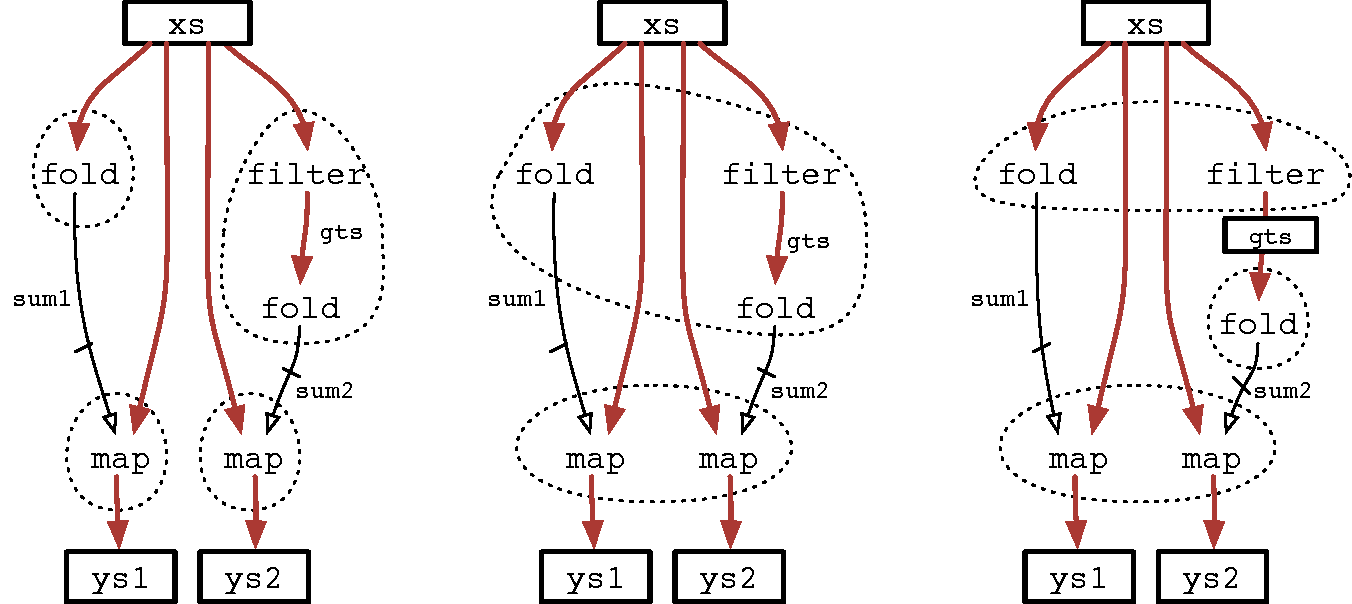
\includegraphics[scale=0.5]{copy/03-body/clustering/figures/ex1-compare.pdf}
\end{center}
\caption{Clusterings for \Hs/normalize2/: with pull streams; our system; best imperative system}
\label{clustering:f:normalize2-clusterings}
\end{figure}


The rightmost diagram in \cref{clustering:f:normalize2-clusterings} shows the clustering determined by the best existing ILP approach for imperative array-based loop fusion.
To obtain this clustering, we first implemented each combinator as a separate imperative loop, shown in \cref{figs/clustering/normalize2-c}.
Imperative clustering algorithms, such as \citet{megiddo1998optimal}, only cluster together loops of the same iteration size.
% The loop that performs the filter operation consumes the array \Hs/xs/, which has size \Hs/xs_length/, and produces the array \Hs/gts/, which has size \Hs/gts_length/.
In the imperative code, the loop that performs the fold over \Hs/gts/ has an iteration size of \Hs/gts_length/, while all the other loops have an iteration size of \Hs/xs_length/.
The final value of \Hs/gts_length/ is not known until the loop that performs the filter completes, so there is a fusion-preventing dependency between the loop that performs the filter and the loop that performs the fold over \Hs/gts/, as well as having different iteration sizes.
The low-level imperative details obscure the high-level meaning of the program, and complicate fusing the filter operation with the subsequent fold.
% The imperative clustering combines the \Hs@sum1@ fold and \Hs@gts@ filter into one loop, as well as combining the two map operations.
% The imperative clustering combines the \Hs@sum1@ fold and \Hs@gts@ filter into one loop, as well as combining the two map operations.
% , but requires an extra loop for the fold operation which consumes the filter output, since it cannot fuse filter operations.

\begin{listing-c}[float,label=figs/clustering/normalize2-c,caption=Unfused imperative implementation of \Hs/normalize2/]
void normalize2(int* xs, size_t xs_length, int* out_ys1, int* out_ys2)
{
    // sum1 = fold (+) 0 xs
    int sum1 = 0;
    for (size_t i = 0; i != xs_length; ++i) {
        sum1 += xs[i];
    }

    // gts = filter ($>$ 0) xs
    int* gts = malloc(sizeof(int) * xs_length);
    size_t gts_length = 0;
    for (size_t i = 0; i != xs_length; ++i) {
        if (xs[i] > 0) {
            gts[gts_length] = xs[i];
            gts_length += 1;
        }
    }

    // sum2 = fold (+) 0 gts
    int sum2 = 0;
    for (size_t i = 0; i != gts_length; ++i) {
        sum2 += gts[i];
    }
    free(gts);

    // ys1 = map (/ sum1) xs
    for (size_t i = 0; i != xs_length; ++i) {
        out_ys1[i] = xs[i] / sum1;
    }

    // ys2 = map (/ sum2) xs
    for (size_t i = 0; i != xs_length; ++i) {
        out_ys2[i] = xs[i] / sum2;
    }
}
\end{listing-c}

Our approach, shown in the middle of \cref{clustering:f:normalize2-clusterings}, produces the optimal clustering in this case: one loop for the filter and folds, another for the maps.
For this example, we could execute each cluster as either push streams (\cref{taxonomy/push}) or as a process network fused by process fusion (\cref{chapter:process:processes}).
In general, a single cluster produced by our algorithm may contain combinators with multiple inputs as well as multiple outputs, so we execute each cluster as a fused process network.

% Data flow fusion~\cite{lippmeier2013data} is a technique to compile a specific class of data flow programs into single, efficient imperative loops. This process of ``compilation'' is equivalent to performing array fusion on a combinator based functional array program, as per related work on stream fusion~\cite{coutts2007stream} and delayed arrays~\cite{keller2010repa}. The key benefits of data flow fusion over this prior work are: 1) it fuses programs that use branching data flows where a produced array is consumed by several consumers, and 2) complete fusion into a single loop is guaranteed for all programs that operate on the same size input data, and contain no fusion-preventing dependencies between operators. This process of ``compilation'' is equivalent to performing array fusion on a combinator based functional array program, as per related work on stream fusion~\cite{coutts2007stream} and delayed arrays~\cite{keller2010repa}. The key benefits of data flow fusion over this prior work are: 1) it fuses programs that use branching data flows where a produced array is consumed by several consumers, and 2) complete fusion into a single loop is guaranteed for all programs that operate on the same size input data, and contain no fusion-preventing dependencies between operators.

% Fusion-preventing dependencies express the fact that some operators simply must wait for others to complete before they can produce their own output. For example, in the following:
% \begin{code}
%   normalize :: Array Int -> Array Int
%   normalize xs = let sum = fold (+) 0 xs
%                  in  map (/ sum) xs
% \end{code}

% If we wish to divide every element of an array by the sum of all elements, then it seems we are forever destined to compute the result using at least two loops: one to determine the sum, and one to divide the elements. The evaluation of @fold@ demands all elements of its source array, and we cannot produce any elements of the result array until we know the value of @sum@. 

% However, many programs \emph{do} contain opportunities for fusion, if we only knew which opportunities to take. The following example offers \emph{several} unique, but mutually exclusive approaches to fusion. \Cref{clustering:f:normalize2-clusterings} on the next page shows some of the possibilities.
% \begin{code}
%  normalize2 :: Array Int -> (Array Int, Array Int)
%  normalize2 xs
%   = let sum1 = fold   (+)  0   xs
%         gts  = filter (> 0)    xs
%         sum2 = fold   (+)  0   gts
%         ys1  = map    (/ sum1) xs
%         ys2  = map    (/ sum2) xs
%     in (ys1, ys2)
% \end{code}

% In \cref{clustering:f:normalize2-clusterings}, the dotted lines show possible clusterings of operators. Stream fusion implicitly choses the solution on the left as its compilation process cannot fuse a produced array into multiple consumers. The best existing ILP approach will chose the solution on the right as it cannot cluster operators that consume arrays of different sizes. Our system choses the solution in the middle, which is also optimal for this example. 

% NOTE: This set of bullets needs to fit on the first page, without spilling to the second.

% We must also decide which clustering is the `best' or most optimal. One obvious criterion for this is the minimum number of loops, but there may even be multiple clusterings with the minimum number of loops. In this case, the number of required manifest arrays must also be taken into account. 

% As real programs contain tens or hundreds of individual operators, performing an exhaustive search for an optimal clustering is not feasible, and greedy algorithms tend to produce poor solutions. 


%!TEX root = ../Main.tex


% -----------------------------------------------------------------------------
\section{Combinator normal form}
\label{clustering:s:CombinatorNormalForm}
To perform clustering on an input program, the program is expressed in \emph{combinator normal form} (CNF), which is a textual description of the dependency graph.
The grammar for CNF is given in \cref{clustering:f:CombinatorNormalForm}.
Syntactically, a CNF program is a restricted Haskell function definition consisting of one or more let-bound array operations.

%!TEX root = ../Main.tex
\begin{figure}
\begin{tabbing}
MMMM        \= MM \= MMMMMMMMM \= \kill
$\scalar$    \> $\to$ \> (scalar variable) \\
$\arrayz$     \> $\to$ \> (array variable)  \\
$f$         \> $\to$ \> (worker function) \\
$\fun$       \> $\to$ \> $f~\scalar\ldots$
\\[2ex]
$\bind$      \> @::=@ \> $\scalar$ \> $=~\sbind$ \\
            \> $~|$  \> $\arrayz$  \> $=~\abind$ \\
            \> $~|$  \> $\scalar\ldots,\arrayz\ldots$ \> $=~@external@~\scalar\ldots~\arrayz\ldots$
\end{tabbing}

\begin{tabbing}
MMMM        \= MM \= MMMMM \= MMMMMM \= M \= MMMM \= MMMMMM \= \kill
$\sbind$     \> @::=@ \> $@fold@$     \> $\fun~~ \arrayz$
\\[1ex]

$\abind$     \> @::=@ \> $@map@_n$    \> $\fun~~ \arrayz^n$ 
            \> $~|$  \> $@filter@$   \> $\fun~~ \arrayz$   \\
            \> $~|$  \> $@generate@$ \> $\scalar~~ \fun$  
            \> $~|$  \> $@gather@$   \> $\arrayz~~ \arrayz$ \\
            \> $~|$  \> $@cross@$    \> $\arrayz~~ \arrayz$
\\[1ex]
$\program$  \> @::=@ \> $f~\scalar\ldots~\arrayz\ldots~=$ \\
            \>          \> $@let@~\bind\ldots$                  \\
            \>          \> $@in@~(\scalar\ldots,~\arrayz\ldots)$
\\[3ex]
@generate@ \= \kill
$@fold@$     \> $:~ (a \to a \to a) \to @Array@~~ a \to a$     \\
$@map@_n$    \> $:~ (\{a_i          \to\}^{\;i\; \gets 1 \dots n}~~ b)  \to
                       \{@Array@~~ a_i \to\}^{\;i\; \gets 1 \dots n}~~ @Array@~~ b$ \\
$@filter@$   \> $:~ (a \to @Bool@) \to @Array@~~ a \to @Array@~~ a$      \\
$@generate@$ \> $:~ @Nat@ \to (@Nat@ \to a) \to @Array@~~ a$          \\
$@gather@$   \> $:~ @Array@~~ a \to @Array@~~ @Nat@  \to @Array@~~ a$ \\
$@cross@$    \> $:~ @Array@~~ a \to @Array@~~ b ~~~~ \to @Array@~~ (a, b)$
\end{tabbing}
\caption{Combinator normal form}
\label{clustering:f:CombinatorNormalForm}
\end{figure}



The \Hs@normalize2@ example from \cref{clustering:s:Introduction} is already in CNF;
its corresponding cluster diagrams are shown in \cref{clustering:f:normalize2-clusterings}.
Our cluster diagrams are similar to Loop Dependence Graphs (LDGs) from related work in imperative array fusion~\cite{gao1993collective}.
We name edges after the corresponding variable from the CNF form, and edges which are fusion preventing are drawn with a dash through them (as per the edge labeled \Hs@sum1@ in \cref{clustering:f:normalize2-clusterings}).
In cluster diagrams, as with dependency graphs, we tend to elide the worker functions to combinators when they are not important to the discussion --- so we don't show the @(+)@ operator on each use of \Hs@fold@.


Clusters of operators, which are to be fused into a single pass by process fusion, are indicated by dotted lines, and we highlight materialized arrays by drawing them in boxes.
In \cref{clustering:f:normalize2-clusterings}, the variables \Hs@xs@, \Hs@ys1@ and \Hs@ys2@ are always in boxes, as these are the material input and output arrays of the program.
In the rightmost cluster diagram, \Hs@gts@ has also been materialized because in this version, the producing and consuming operators (\Hs@filter@ and \Hs@fold@) have not been fused together.
In the grammar given in \cref{clustering:f:CombinatorNormalForm}, the bindings have been split into those that produce scalar values ($sbind$), and those that produce array values ($abind$).
In the cluster diagrams of \cref{clustering:f:normalize2-clusterings}, scalar values are represented by open arrowheads, and array values are represented by closed arrowheads.

%What's a 'suggestive' type???
Most of our array combinators are standard.
Although not part of the grammar, we give the type of each combinator at the bottom of \cref{clustering:f:CombinatorNormalForm}.
The $\Hs@map@_n$ combinator takes a worker function, $n$ arrays of the same length, and applies the worker function to all elements at the same index.
As such, it is similar to Haskell's \Hs@zipWith@, with an added length restriction on the argument arrays.
The \Hs@generate@ combinator takes an array length and a worker function, and creates a new array by applying the worker to each index.
The \Hs@gather@ combinator takes an array of elements, an array of indices, and produces the array of elements that are positioned at each index.
In Haskell, \Hs@gather@ would be implemented as (\Hs@gather arr ixs = map (index arr) ixs@).
The \Hs@cross@ combinator returns the cartesian product of two arrays. 

The exact form of the worker functions is left unspecified, as it is not important for the discussion.
We assume that workers are pure, can at least compute arithmetic functions of their scalar arguments, and index into arrays in the environment.
We also assume that each CNF program considered for fusion is embedded in a larger host program which handles file IO and the like.
Workers are additionally restricted so they can only directly reference the \emph{scalar} variables bound by the local CNF program, though they may reference array variables bound by the host program.
All access to locally bound array variables is via the formal parameters of array combinators, which ensures that all data dependencies we need to consider for fusion are explicit in the dependency graph.

The \Hs@external@ binding invokes a host library function that can produce and consume arrays, but cannot be fused with other combinators.
All arrays passed to and returned from host functions are fully materialised.
External bindings are explicit \emph{fusion barriers}, which force arrays and scalars to be fully computed before continuing. 

Finally, note that \Hs@filter@ is only one representative size-changing operator.
We can handle other combinators, such as \Hs@unfold@ and \Hs@slice@, in our framework, but we stick with simple filtering to aid the discussion.
We discuss other combinators in \cref{clustering:s:FutureWork}.


%!TEX root = ../Main.tex
\section{Size inference}
The array operations in a cluster are fused together into a loop with a specific number of iterations.
Array operations that process different sized arrays cannot usually be assigned to the same cluster, because they require different sized loops.
Consumers of arrays produced by size-changing operations can be assigned to the same cluster as operations that process different sized arrays, but only in specific circumstances, which we shall see in \cref{clustering/size/transducers}.
Before performing clustering, we need to infer the relative sizes of each array in the program, as the sizes determine the relative loop sizes of each array operation, and whether they can be assigned to the same cluster.
We use a simple constraint-based inference algorithm.
Size inference has been previously described in the context of array fusion by \citet{chatterjee1991size}.
In constrast to our algorithm, \citet{chatterjee1991size} does not support size-changing functions such as filter.

Although our constraint-based formulation of size inference is reminiscent of type inference for HM(X)~\cite{odersky1999type}, there are important differences.
Firstly, our type schemes include existential quantifiers, which express the fact that the sizes of arrays produced by filter operations are statically unknown, in general.
The output size of \Hs@generate@ is also statically unknown, as the result size is data-dependent and is not available until runtime.
HM(X) style type inferences use the $\exists$ quantifier to bind local type variables in constraints, and existential quantifiers do not appear in type schemes.
Secondly, our types are first-order only, as program graphs cannot take other program graphs as arguments.
Provided we generate the constraints in the correct form, solving them is straightforward.

Size inference cannot statically infer array sizes for all programs.
The $\Hs/map/_n$ combinator requires all input arrays to be the same size, and returns an output array of the same size.
Compared to \Hs/zipWith/, which returns a statically unknown size, this extra restriction gives size inference more information about the size of the output array, which in turn may allow more array operations to be assigned to the same cluster.
If we cannot statically determine that all input arrays given to $\Hs/map/_n$ are the same size, size inference will fail: the program may still be compiled, but fusion is not performed.

% -----------------------------------------------------------------------------
\begin{figure}
\begin{tabbing}
MMMMMMMMM \= MM  \= MM \= MMMMMM \= \kill
\textbf{Size Type}
\> $\tau$   \> @::=@  \> $k$                  \> (size variable)       \\
\>          \> $~|$   \> $\tau \times \tau$   \> (cross product)
\end{tabbing}

\begin{tabbing}
MMMMMMMMM \= MM  \= MM \= MMMMMM \= \kill
\textbf{Size Constraint}
\> $C$      \> @::=@  \> $\true$               \> (trivially true)      \\
\>          \> $~|$   \> $k = \tau$           \> (equality constraint) \\
\>          \> $~|$   \> $C \wedge C$         \> (conjunction)
\end{tabbing}

\begin{tabbing}
MMMMMMMMM \= MM  \= MM \= MMMMMM \= \kill
\textbf{Size Scheme}
\> $\sigma$ \> @::=@  
        \> $\forall \ov{k}.~ \exists \ov{k}.~ (\ov{ x : \tau }) \to (\ov{x : \tau})$
\end{tabbing}

\caption{Sizes, constraints and schemes}
\label{clustering:f:constraints}
\end{figure}


\newcommand{\constr}[1]{\llbracket #1 \rrbracket}


% -----------------------------------------------------------------------------
\subsection{Size types, constraints and schemes}
\label{clustering:s:SizeTypes}
\Cref{clustering:f:constraints} shows the grammar for size types, constraints and schemes.
A size scheme is like a type scheme from Hindley-Milner style type systems, except that it only mentions the size of each input array, and ignores the element types.

A size may either be a variable $k$ or a cross product of two sizes.
We use the latter to represent the result size of the \Hs@cross@ operator discussed in the previous section.
Constraints may either be trivially $\true$, an equality $k = \tau$, or a conjunction of two constraints $C \wedge C$.
We refer to the trivially true and equality constraints as \emph{atomic constraints}.
Size schemes relate the sizes of each input and output array.
The \Hs@normalize2@ example from \cref{clustering:f:normalize2-clusterings}, which returns two output arrays of the same size as the input, has the following size scheme:
% For example, the size scheme for the \Hs@normalize2@ example from \cref{clustering:f:normalize2-clusterings}, which returns two arrays of the same size as the input, is as follows:
$$
\Hs@normalize2@ ~:_s \forall k.~ (xs : k) \to (ys_1 : k,~ ys_2 : k)
$$

We write $:_s$ to distinguish size schemes from type schemes.

The existential quantifier appears in size schemes when the array produced by a filter or generate appears in the result.
For example:

\begin{haskell}
filterLeft %\(:\sb{s}\,\forall\,k\sb{1}.\,\exists\,k\sb{2}.\,(xs\,:\,k\sb{1})\;\to\;(ys\sb{1}\,:\,k\sb{1},\,ys\sb{2}\,:\,k\sb{2})\)%
filterLeft xs
  = let ys1 = map (+ 1)   xs
        ys2 = filter even xs
    in (ys1, ys2)
\end{haskell}

The size scheme of \Hs@filterLeft@ shows that it works for input arrays of all sizes.
The first result array has the same size as the input, and the second has some statically unknown size.

Finally, note that size schemes form only one aspect of the type information that would be expressible in a full dependently typed language.
For example, in Coq or Agda we could write something like:

\begin{haskell}
filterLeft : %\(\forall\,k\sb{1}:\,\)Nat\(.~\,\exists\,k\sb{2}:\,\)Nat\(.\)% Array %\(k\sb{1}\)% Float -> (Array %\(k\sb{1}\)% Float, Array %\(k\sb{2}\)% Float)
\end{haskell}

However, the type inference systems for fully higher order dependently typed languages typically require quantified types to be provided by the user, and do not perform the type generalization process.
In our situation, we need automatic type generalization, but for a first-order language only.


%!TEX root = ../Main.tex

\begin{figure*}
\footnotesize
% -------------------------------------------------------------------
$$
\fbox{$
 \SizeL {\Gamma}
        {\textit{lets}}
        {\Gamma}
        {C}
$}
$$
%
$$
\ruleI{}{
        \SizeL  {\Gamma}
                {@let@ ~\cdot~ @in@~ exp}
                {\Gamma}
                {\true}
}
\quad
\textrm{(SNil)}
$$

$$
\ruleI  {\SizeB {\Gamma_1}
                {zs}
                {b}
                {\Gamma_2}
                {C_1}
         \quad
         \SizeL {\Gamma_2}
                {@let@~ bs~ @in@~ exp}
                {\Gamma_3}
                {C_2}
        }
        {\SizeL {\Gamma_1}
                {@let@~ zs~ = b~ ;~ bs~ @in@~ exp}
                {\Gamma_3}
                {C_1 \wedge C_2}
        }
\quad
\textrm{(SCons)}
$$

% -------------------------------------------------------------------
$$
\fbox{$ 
 \SizeB {\Gamma}
        {z}
        {bind}
        {\Gamma}
        {C}
$}
$$
%
$$
\begin{array}{lllll}
% map_n
\SizeB  {\Gamma[xs_i : k_i]^{i \gets 1..n}       &}
        {zs}
        {@map@_n~ f~ \{xs_i\}^{i \gets 1..n}     &}
        {\Gamma,~ zs : k_{zs},~ k'               &}
        {\bigwedge_{i \gets 1..n}
                \{k_i = k'\}
         ~\wedge~ k_{zs} = k'}
\\[1ex]

% filter
\SizeB  {\Gamma                                 &}
        {zs}
        {@filter@~ f~ xs                        &}
        {\Gamma,~ zs : k_{zs},~ \exists k'      &}
        {k_{zs} = k'}
\\[1ex]

% fold
\SizeB  {\Gamma                                 &}
        {x~}
        {@fold@~ f~ xs                          &}
        {\Gamma                                 &}
        {\true}
\\[1ex]

% generate
\SizeB  {\Gamma                                 &}
        {zs}
        {@generate@~ s~ f                       &}
        {\Gamma,~ zs : k_{zs},~ \exists k'      &}
        {k_{zs} = k'}
        \\[1ex]

% gather
\SizeB  {\Gamma[is : k_{is}]                    &}
        {zs}
        {@gather@~ xs~ is                       &}
        {\Gamma,~ zs : k_{zs},~ k'              &}
        {k_{zs} = k',~ k_{is} = k'}
\\[1ex]

% cross
\SizeB  {\Gamma[xs : k_{xs},~ ys : k_{ys}]      &}
        {zs}
        {@cross@~ xs~ ys                        &}
        {\Gamma,~ zs : k_{zs},~ k',~ k''        &}
        {k_{zs} = k' \times k'' 
                ~\wedge~ }
\\
& & & \quad\ \  k_{xs} = k' ~\wedge~ k_{ys} = k''
\\[1ex]

% external
\SizeB  {\Gamma                                 &}
        {zs}
        {@external@~ \{xs\}^{i \gets 1..n}      &}
        {\Gamma,~ zs : k_{zs},~ \exists k'      &}
        {k_{zs} = k'}
\end{array}
$$

\caption{Constraint generation for size inference}
\label{clustering:f:ConstraintGeneration}
\end{figure*}


% -----------------------------------------------------------------------------
\subsection{Constraint generation}
The rules for constraint generation are shown in \cref{clustering:f:ConstraintGeneration}.
The first judgment form is written as ($\SizeL{\Gamma_1}{\textit{lets}}{\Gamma_2}{C}$) and reads: ``under environment $\Gamma_1$, the bindings in $\textit{lets}$ produce the result environment $\Gamma_2$ and size constraints $C$''.

\pagebreak
The second judgment form ($\SizeB{\Gamma_1}{zs}{b}{\Gamma_2}{C}$) performs constraint generation for a single binding and reads: ``under environment~$\Gamma_1$, array or scalar variable $zs$ binds the result of combinator application $b$, producing a result environment $\Gamma_2$ and size constraints $C$''.
The environment ($\Gamma$) has the following grammar:
$$
\Gamma~ @::=@ ~~\cdot ~~|~~ \Gamma,~ \Gamma ~~|~~ zs : k ~~|~~ k ~~|~~ \exists k
$$

As usual, ($\cdot$) represents the empty environment and ($\Gamma,~ \Gamma$) represents environment concatenation.
The element ($zs : k$) records the size $k$ of some array variable $zs$.
A plain $k$ indicates that $k$ can be unified with other size types when solving constraints, whereas $\exists k$ indicates a  \emph{rigid} size variable that cannot be unified with other sizes.
We use the $\exists k$ syntax because this variable will also be existentially quantified if it appears in the size scheme of the overall program.

The constraints are generated in a specific form in \cref{clustering:f:ConstraintGeneration}, to facilitate the constraint solving process.
For each array variable in the program, we generate a new size variable, like size $k_{zs}$ for array variable $zs$.
These new size variables always appear on the \emph{left} of atomic equality constraints.
For each array binding, we may also introduce unification or rigid variables; these appear on the \emph{right} of atomic equality constraints.

The final environment and constraints generated for the \Hs@normalize2@ example from \cref{clustering:s:Introduction} are as follows, with the program shown on the right:

\begin{minipage}{0.5\textwidth}
$$
\begin{array}{ll}
   & @xs @ : k_{xs},~
\\ & @gts@ : k_{gts},~ \exists k_1,
\\ & @ys1@ : k_{ys1},~ k_2,
\\ & @ys2@ : k_{ys2},~ k_3
\\
\vdash & \true 
        ~\wedge~  k_{gts} = k_1
\\ \wedge & \true
        ~ \wedge~  k_{xs}  ~= k_2
        ~ \wedge~  k_{ys1}  = k_2 
\\     &~~~~~~~\; 
          \wedge~  k_{xs}   = k_3
        ~ \wedge~  k_{ys2}  = k_3
\end{array}
$$
\end{minipage}
\begin{minipage}{0.5\textwidth}
% normalize2 %\(:_s \forall k_{xs}.~ (xs : k_{xs}) \to (ys_1 : k_{xs},~ ys_2 : k_{xs})\)%
\begin{haskell}
normalize2 xs
 = let sum1 = fold   (+)  0   xs
       gts  = filter (>   0)  xs
       sum2 = fold   (+)  0   gts
       ys1  = map    (/ sum1) xs
       ys2  = map    (/ sum2) xs
   in (ys1, ys2)
\end{haskell}
\end{minipage}

To compute the constraints and environment for this example, the input environment given to constraint generation records that the input array \Hs/xs/ has the corresponding size type $k_{xs}$.
This input environment is described in \cref{clustering:s:ConstraintSolvingGen}.
For each binding, the rules in \cref{clustering:f:ConstraintGeneration} generate a constraint and add any required array and size bindings to the environment.
The \Hs/sum1/ binding, a \Hs/fold/, does not bind any array variables and works for any input size, so the corresponding rule leaves the environment as-is and produces a $\true$ constraint.
For the \Hs/gts/ binding, a \Hs/filter/, the size of the output array is unknown.
The \Hs/filter/ rule records the size of the output array by introducing a new size-type variable $k_{gts}$, as well as an existential variable $k_1$; the rule also generates the constraint ($k_{gts} = k_1$).
For the \Hs/ys1/ binding, a \Hs/map/, the size of the output array is the same as the input array.
The \Hs/map/ rule introduces a new size variable $k_{ys1}$ to record the size of the output array, and introduces a new unification variable $k_2$.
The rule introduces constraints requiring the new unification variable $k_2$ to be equal to both the input size variable $k_{xs}$ and the output size variable $k_{ys1}$.
In the constraints, array size variables occur on the left-hand side and unification variables occur on the right-hand side.
Constraint generation for the remaining bindings proceeds similarly.


% -------------------------------------------------------------------
\subsection{Constraint solving and generalization}
\label{clustering:s:ConstraintSolvingGen}
\Cref{clustering:f:ConstraintSolving} shows the rule for assigning a size scheme to a program.
The top-level judgment form ($\SizeF{\program}{\sigma}$) assigns size scheme $\sigma$ to $\program$.

%!TEX root = ../Main.tex

\newcommand\ins{\textit{ins}}
\newcommand\inty{\textit{inty}}
\begin{figure*}
\footnotesize
$$
\fbox{$
 \SizeF {\program}{\sigma}
$}
$$
$$
\ruleI  {
          \SizeL{\Gamma_0}
                {@let@~ bs~ @in@~ \{ ys_j \}^{j \gets 1 .. m}}
                {\Gamma_1}{C_1}
\qquad
  (\Gamma_2,C_2) = \textrm{SOLVE}(\Gamma_1,~ C_1)
  \qquad
          \forall k \in \textrm{fv}(\ov{s}).~
          (\exists k) \notin \Gamma_2
        }
        {
        \begin{array}{c}
        \SizeF{f~ \{xs\}^{i \gets 1..n}
                        = @let@~ bs~ @in@~ \{ys\}^{j \gets 1..m}
                }
                { \forall \overline{k_a}.~ 
                  \exists \overline{k_e}.~
                        (\{ xs_i : s_i \}^{i \gets 1..n}) \to
                        (\{ ys_j : t_j \}^{j \gets 1..m})
                }
\\[1em]
\begin{array}{lll}
\mbox{where }
  & \Gamma_0 & = \{k_i,~ xs_i : k_i \}^{ i \gets 1 .. n }
\\
\\
  & \ov{s} & = \{ s_i ~|~ i \in 1..n  ~\wedge~ (k_i = s_i) \in C_2 \}
\\
 & \ov{k'} & = \{ k'_j ~|~ j \in 1..m ~\wedge~ (ys_j : k_j') \in \Gamma_2 \}
\\
  & \ov{t} & = \{ t_j ~|~ j \in 1..m  ~\wedge~ (k_j' = t_j ) \in C_2 \}
\\
\\
 & \ov{k_a} & = \{ k ~|~ k         \in \Gamma_2 ~\wedge~ k \in \textrm{fv}(\ov{s}) \}  
%                        ~\cap~ (\bigcup_{i \gets 1 .. n}\textrm{fv}(s_i))
\\
 & \ov{k_e} & = \{ k ~|~ \exists k \in \Gamma_2 ~\wedge~ k \in \textrm{fv}(\ov{t}) \}
%                        ~\cap~ (\bigcup_{j \gets 1 .. m}\textrm{fv}(t_j))
\end{array}
\end{array}
        }
\quad
\textrm{(SProgram)}
$$

\caption{Constraint solving for size inference}
\label{clustering:f:ConstraintSolving}
\end{figure*}



Rule (SProgram) assigns a size scheme to a program by first extracting size constraints, before solving them and generalizing the result.
In the rule, $\Gamma_0$ is used as the input environment to constraint generation, and is constructed by generating a fresh size variable ($k_i$) for each input array ($xs_i$).
The environment and constraints produced by constraint generation are named $\Gamma_1$ and $C_1$; these constraints are then solved using the $\textrm{SOLVE}$ function, which we describe soon.
The constraints, after being solved, are stored in $C_2$, and the environment in $\Gamma_2$.
We use the solved constraints to find the size types of the input arrays ($\ov{s}$), and the size types of the output arrays ($\ov{t}$).
We perform generalization by adding universal quantifiers for the unification variables mentioned by the types of input arrays ($\ov{k_a}$), and adding existential quantifiers for the existential variables mentioned by the types of output arrays ($\ov{k_e}$).
Finally, we require that the types of input arrays do not mention any existential variables; an example of this restriction is shown in \cref{clustering:s:RigidSizes}.

In the rule, the solving process is indicated by $\textrm{SOLVE}$, and takes an environment and a constraint set, and produces a solved environment and constraint set.
As the constraint solving process is both standard and straightforward, we only describe it informally.

During constraint generation in the previous section, we were careful to ensure that all the size variables named after program variables are on the left of atomic equality constraints, while all the unification and existential variables are on the right.
To solve the constraints, we keep finding pairs of atomic equality constraints where the same variable appears on the left, unify the right of both of these constraints, and apply the resulting substitution to both the environment and original constraints.
When there are no more pairs of constraints with the same variable on the left, the constraints are in solved form and we are finished.

During constraint solving, all unification variables occuring in the environment can have other sizes substituted for them.
In contrast, the rigid variables marked by the $\exists$ symbol cannot.
For example, consider the constraints for \Hs@normalize2@ mentioned before:
$$
\begin{array}{ll}
   & @xs @ : k_{xs},~
@gts@ : k_{gts},~ \exists k_1,~
@ys1@ : k_{ys1},~ k_2,~
@ys2@ : k_{ys2},~ k_3
\\
\vdash & \true 
        ~\wedge~  k_{gts} = k_1 ~\wedge~ \true
\\     &~~~~~~~\; 
          \wedge~  \colorbox{Highlighted}{$k_{xs}  ~= k_2$}
          \wedge~  k_{ys1}  = k_2 
\\     &~~~~~~~\; 
        ~ \wedge~  \colorbox{Highlighted}{$k_{xs}   = k_3$}
        ~ \wedge~  k_{ys2}  = k_3
\end{array}
$$

In the highlighted constraints, $k_{xs}$ is mentioned twice on the left of an atomic equality constraint, so we can substitute $k_2$ for $k_3$. Eliminating the duplicates, as well as the trivially $\true$ terms then yields:
$$
\begin{array}{ll}
   & @xs @ : k_{xs},~
@gts@ : k_{gts},~ \exists k_1,~
@ys1@ : k_{ys1},~ k_2,~
@ys2@ : k_{ys2},~ k_3
\\
\vdash & k_{gts} = k_1
        ~\wedge~  k_{xs}  ~= k_2
        ~\wedge~  k_{ys1}  = k_2 
        ~\wedge~  k_{ys2}  = k_2
\end{array}
$$

To produce the final size scheme, we look up the sizes of the input and output variables of the original program from the solved constraints and generalize appropriately.
This process is determined by the top-level rule in \cref{clustering:f:ConstraintSolving}.
In the case of \Hs/normalize2/, no rigid size variables appear in the result, so we can universally quantify all size variables to get the following size scheme:
$$\Hs@normalize2@ ~:_s \forall k_2. (xs : k_2) \to (ys_1 : k_2,~ ys_2 : k_2)
$$


Rule~(SProgram) also characterises the programs we accept: a program is \emph{valid} if and only if $\exists \sigma.\ \SizeF{\program}{\sigma}$. 

% -----------------------------------------------------------------------------
\subsection{Rigid sizes}
\label{clustering:s:RigidSizes}
When the environment of our size constraints contains rigid variables (indicated by $\exists k$), we introduce existential quantifiers instead of universal quantifiers into the size scheme.
Consider the \Hs@filterLeft@ program from \cref{clustering:s:SizeTypes}:
\begin{haskell}
filterLeft xs
 = let ys1 = map (+ 1)   xs
       ys2 = filter even xs
   in (ys1, ys2)
\end{haskell}

The size constraints for this program, already in solved form, are as follows:
$$
\begin{array}{ll}
       & xs : k_{xs},~ ys_1 : k_{ys1},~ k_1,~ ys_2 : k_{ys2},~ \exists k_2
\\
\vdash &          k_{xs}   = k_1
        ~\wedge~  k_{ys_1} = k_1 
        ~\wedge~  k_{ys_2} = k_2
\end{array}
$$

As variable $k_2$ is marked as rigid, we introduce an existential quantifier for it, producing the size scheme stated earlier:

$$
@filterLeft@ :\sb{s}\,\forall k\sb{1}.\ \exists k\sb{2}.\ (xs\,:\,k\sb{1})\;\to\;(ys\sb{1}\,:\,k\sb{1},\,ys\sb{2}\,:\,k\sb{2})
$$

Note that, although rule~(SProgram) from \cref{clustering:f:ConstraintSolving} performs a \emph{generalization} process, there is no corresponding instantiation rule.
The size inference process works on the entire graph at a time, and there is no mechanism for one operator to invoke another.
To say this another way, all subgraphs are fully inlined.
Recall from \cref{clustering:s:CombinatorNormalForm} that we assume our operator graphs are embedded in a larger host program.
We use size information to guide the clustering process, and although the host program can certainly call the operator graph, static size information does not flow across this boundary.

When producing size schemes, we do not permit the arguments of an operator graph to have existentially quantified sizes.
This restriction is necessary to reject programs that we cannot statically guarantee will be well-sized.
For example:
\begin{haskell}
bad1 xs
 = let flt = filter p xs
       ys  = map2   f flt xs
   in  ys
\end{haskell}

The above program filters its input array, and then applies \Hs@map2@ to the filtered version as well as the original array.
As the \Hs@map2@ operator requires both of its arguments to have the same size, \Hs@bad1@ would only be valid when the predicate \Hs@p@ is always true.
We could execute this program as a process network if we replaced the \Hs/map2/ operator with \Hs/zipWith/, and explicitly read from the input array \Hs/xs/ twice, as in the two-source version of \Hs/partitionAppend/ from \cref{s:Benchmarks:partitionAppend}.
The result size of the \Hs/zipWith/ operator is the smaller of the two input operators; the extra size restriction on \Hs/map2/ simplifies size inference, as we do not need to introduce the concept of the minimum of size types.
The size constraints for \Hs/bad1/ are as follows:
$$
\begin{array}{ll}
       & xs : k_{xs},~ \mi{flt} : k_{\mi{flt}},~ \exists k_1,~ ys : k_{ys},~ k_2
\\
\vdash &          k_{\mi{flt}}  = k_1
        ~\wedge~  k_{\mi{flt}}  = k_2
        ~\wedge~  k_{xs}   = k_2
        ~\wedge~  k_{ys}   = k_2
\end{array}
$$

Solving these constraints then yields:

$$
\begin{array}{ll}
       & xs : k_{xs},~ \mi{flt} : k_{\mi{flt}},~ \exists k_1,~ ys : k_{ys},~ k_1
\\
\vdash &          k_{\mi{flt}}  = k_1
        ~\wedge~  k_{xs}   = k_1
        ~\wedge~  k_{ys}   = k_1
\end{array}
$$

In this case, rule~(SProgram) does not apply, because the parameter variable $xs$ has size $k_1$, but $k_1$ is marked as rigid in the environment (with $\exists k_1$). 
This function is rejected by size inference, as a caller cannot guarantee that an input array's size matches the existential size type chosen by the function.

As a final example, the following program is ill-sized because the two filter operators are not guaranteed to produce the same number of elements:
\begin{haskell}
bad2 xs
 = let flt1 = filter p1 xs
       flt2 = filter p2 xs
       ys   = map2   f  flt1 flt2
   in  ys
\end{haskell}

The initial size constraints for this program are:
\newcommand\flt{\textit{flt}}
$$
\begin{array}{ll}
       & xs : k_{xs},~ \flt1 : k_{\flt1},~ \exists k_1,~ \flt2 : k_{\flt2},~ \exists k_2,~ ys : k_{ys},~ k_3
\\
\vdash &          k_{\flt1}   = k_1
        ~\wedge~  k_{\flt2}   = k_2
        ~\wedge~  k_{\flt1}   = k_3
        ~\wedge~  k_{\flt2}   = k_3
        ~\wedge~  k_{ys}   = k_3
\end{array}
$$

To solve these, we note that $k_{\flt1}$ is used twice on the left of an atomic equality constraint, so we substitute $k_1$ for $k_3$:
$$
\begin{array}{ll}
       & xs : k_{xs},~ \flt1 : k_{\flt1},~ \exists k_1,~ \flt2 : k_{\flt2},~ \exists k_2,~ ys : k_{ys},~ k_1
\\
\vdash &          k_{\flt1}   = k_1
        ~\wedge~  k_{\flt2}   = k_2
        ~\wedge~  k_{\flt2}   = k_1
        ~\wedge~  k_{ys}   = k_1
\end{array}
$$

At this stage we are stuck, because the constraints are not yet in solved form, and we cannot simplify them further.
Both $k_1$ and $k_2$ are marked as rigid, so we cannot substitute one for the other and produce a single atomic constraint for $k_{\flt2}$.
The $\textrm{SOLVE}$ function fails to return a solution, and rule (SProgram) cannot apply.

% The \Hs/bad2/ example is similar to the \Hs/partitionAppend/ example from \cref{s:Benchmarks}, where the input stream is filtered twice, and both results are appended together.
% We were able to execute \Hs/partitionAppend/ as a streaming process by 

% \newcommand{\eqclasses}[1]{
%     \begin{tabbing}
%         MM \= M \= \kill
%         #1
%     \end{tabbing}}
% 
% \newcommand{\eqclass}[2]{$#1$ \> $\in$ \> $\{#2\}$ \\}

% The next example involves two filters using the same predicate.
% Despite using the same predicate and input data, we produce different output sizes for each filter.
% \begin{tabbing}
% @MMMMMMMMMMMMMMMMMMMMMMMMMMMMMMMM@  \= \kill
% @diff xs@                           \> $\exists k_{xs}.$ \\
% @ = let ys1 = filter p xs@          \> $\forall k_{ys1}.$       \\
% @       ys2 = filter p xs@          \> $\forall k_{ys2}.$       \\
% @   in (ys1, ys2)@                  \> $true$                   \\
% \end{tabbing}
% 
% This constraint is valid, with the equivalence classes being:
% \eqclasses{
%     \eqclass{k_{xs}}    {k_{xs}}
%     \eqclass{k_{ys1}}   {k_{ys1}}
%     \eqclass{k_{ys2}}   {k_{ys2}}
% }


% -----------------------------------------------------------------------------
\subsection{Iteration size}
After inferring the size of each array variable, each operator is assigned an \emph{iteration size}, which is the number of iterations needed in the loop that evaluates the operator.
For \Hs@filter@ and other size-changing operators, the iteration and result sizes are in general different.
For such an operator, we say that the result size is a \emph{descendant} of the iteration size.
Conversely, the iteration size is a \emph{parent} of the result size. 

This descendant--parent size relation is transitive, so if we filter an array, then filter the resulting array, the size of the result is a descendant of the iteration size of the initial filter.
This relation arises naturally from the fact that we compile individual clusters into a single process using process fusion (\cref{chapter:process:processes}).
With process fusion, such an operation would be compiled into a process containing a single loop that pulls from a stream backed by the input array --- with an iteration size identical to the size of the input array, and containing two case instructions to perform the two layers of filtering.

Iteration sizes are used to decide which operators can be fused with each other.
As in prior work, operators with the same iteration size can be fused.
However, in prior work, operators with different iteration size cannot be assigned to the same cluster, as imperative loop fusion systems cannot generally fuse loops of different iteration sizes.
In our system, we also allow operators of different iteration sizes to be fused, provided those sizes are descendants of the same parent size.

\begin{figure}
\begin{tabbing}
MMMMM \= M \= MMMMMMMMMM \= MM \= \kill
$\iiter_{\Gamma,C}$  
        \>$:$\> $\bind \rightarrow T$ 
\\[1ex]
$\iiter_{\Gamma,C}$
        \> $|$  \> $(z~ = \Hs@fold@~ f~xs)$     
                \> $=$ \> $C(\Gamma(xs))$ 
\\
        \> $|$  \> $(ys = \Hs@map@_n~f~\overline{xs})$
                \> $=$ \> $C(\Gamma(ys))$ 
\\
        \> $|$  \> $(ys = \Hs@filter@~f~xs)$    
                \> $=$ \> $C(\Gamma(xs))$ 
\\
        \> $|$  \> $(ys = \Hs@generate@~s~f)$  
                \> $=$ \> $C(\Gamma(ys))$ 
\\
        \> $|$  \> $(ys = \Hs@gather@~is~xs)$    
                \> $=$ \> $C(\Gamma(is))$ 
\\
        \> $|$  \> $(ys = \Hs@cross@~as~bs)$     
                \> $=$ \> $C(\Gamma(as)) \times C(\Gamma(bs))$ 
\\
        \> $|$  \> $(ys = \Hs@external@~\overline{xs})$  
                \> $=$ \> $\bot$ 
\end{tabbing}
\caption{Computing the iteration size of a binding}
\label{fig:clustering:iter}
\end{figure}


We use $T$ to range over iteration sizes, and write $\bot$ for the case where the iteration size is unknown. The $\bot$ size is needed to handle the \Hs@external@ operator, as we cannot statically infer its true iteration size, and it cannot be fused with any other operator.

\begin{tabbing}
MMMMMMMM \= MM       \= MM \= MMMM \= \kill
\textbf{Iteration Size}
 \> $T$         \> @::=@  \> $\tau$        \> (known size) \\
 \>             \> $~|$   \> $\bot$     \> (unknown size) \\
\end{tabbing}

Once the size constraints have been solved, we can use the $\iiter$ function in \cref{fig:clustering:iter} to compute the iteration size of each binding.
In the definition, we use the syntax $\Gamma(xs)$ to find the ($xs : k$) element in the environment $\Gamma$ and return the associated size $k$.
Similarly, we use the syntax $C(k)$ to find the corresponding ($k = \tau$) constraint in $C$ and return the associated size type $\tau$.


% Once the constraints are solved, known to be valid, and sorted into equivalence classes, each combinator is assigned a size. Note that for a filter, the size of the output array $k_o$ is some existential that is less than or equal to $k_n$, but the actual loop size of the \emph{combinator} is equal to $k_n$. This is because, in order to produce the filtered output, all elements of the input $n$ must be considered.

% After the generated equality constraints are solved, and sizes are grouped into equivalence classes, combinators with iteration sizes in the same equivalence class may be fused together if there are no fusion-preventing dependencies between them.


% -----------------------------------------------------------------------------
\subsection{Transducers and compatible common ancestors}
\label{clustering/size/transducers}
%     we've said that several times before
% Unlike previous work, we do allow combinators with different iteration sizes to be fused together. For example, an operation on filtered data may be fused with the filter operation that generates the data, even though the iteration sizes are different.

\begin{figure}
\begin{tabbing}
MMMM \= MM \= MMMMMMMMM \= MMMM \= MM \= \kill
$\trans$  \>$:$\> $\{\bind\} \rightarrow \name \rightarrow \{\name\}$ \\
$\trans(bs,o)$    \\
            \> $|$ \> $o = \Hs@filter@~f~n$    \> $\in bs$ \> $=$ \> $\trans'(bs,n)$ \\
            \> $|$ \> otherwise             \>          \> $=$ \> $\trans'(bs,o)$ \\
\\
$\trans'(bs,o)$    \\
            \> $|$ \> $o = \Hs@fold@~f~n$      \> $\in bs$ \> $=$ \> $\emptyset$ \\
            \> $|$ \> $o = \Hs@map@_n~f~ns$    \> $\in bs$ \> $=$ \> $\bigcup_{x \in ns} \trans(bs, x)$ \\
            \> $|$ \> $o = \Hs@filter@~f~n$    \> $\in bs$ \> $=$ \> $\{o\}$       \\
            \> $|$ \> $o = \Hs@generate@~s~f$  \> $\in bs$ \> $=$ \> $\emptyset$ \\
            \> $|$ \> $o = \Hs@gather@~i~d$    \> $\in bs$ \> $=$ \> $\trans(bs,i)$ \\
            \> $|$ \> $o = \Hs@cross@~a~b$     \> $\in bs$ \> $=$ \> $\emptyset$ \\
            \> $|$ \> $o = \Hs@external@~ins$  \> $\in bs$ \> $=$ \> $\emptyset$ \\
\end{tabbing}
\caption{Finding the parent transducers of a combinator}
\label{fig:clustering:trans}
\end{figure}

We define the concept of \emph{transducers} as combinators having a different output size to their iteration size.
As with any other combinator, a transducer may fuse with other combinators of the same iteration size, but transducers may also fuse with combinators having iteration size the same as the transducer's output size.
For our set of combinators, the only transducer is \Hs@filter@.

Looking back at the \Hs@normalize2@ example, most combinators consume the input array \Hs/xs/, and so have an iteration size of $k_{xs}$.
The filter that consumes the \Hs/xs/ array and produces the differently-sized \Hs/gts/ array is a transducer from $k_{xs}$ to $k_{gts}$.
The fold that consumes the output of the filter has an iteration size of $k_{gts}$.
This fold can be fused with its parent transducer, the filter combinator, despite the two having different iteration sizes.

\Cref{fig:clustering:trans} defines a function $\trans$, to find the parent transducer of a combinator application.
Since each name is bound to at most one combinator, we abuse terminology here slightly and write \emph{combinator $n$} when refering to the combinator occuring in the binding of the name $n$.
The parent transducer $\trans(bs, n)$ of a combinator $n$ has the same output size as $n$'s iteration size, but the two have different iteration sizes.
Although the input program's dependency graph forms a directed acyclic graph, the relationship between the combinators in the graph and each combinator's respective parent transducer, if it has one, forms a forest.

With the $\trans$ function, we can express the restriction on programs we view as valid for clustering as the following:

\textbf{Definition: sole transducers}.
If a program $p$ is \emph{valid}, then its bindings will have at most one transducer:
\[
\forall p, \sigma, n.\ \ \ \ p :_s \sigma \implies |\trans(\mi{binds}(p), n)| \le 1
\]

Intuitively, we can see that this restriction holds for programs on which size inference succeeds.
By inspecting the definition of $\trans'$ and performing case analysis on the combinator binding, we see that only the $\Hs/map/_n$ clause in $\trans'$ can return multiple transducers, and only the \Hs/filter/ clause directly returns a transducer.
Since the constraint generation for $\Hs/map/_n$ requires all inputs to have the same size, the inputs will also have the same transducer.
If the inputs had different transducers, then their size would be generated by different filters, and each would have its own separate existential variable as a size type, not fulfilling the same-size requirement for $\Hs/map/_n$.

% \textbf{Proof:} by induction on $bs$. If $n = \Hs@map@_n~f~ns$,
% then $trans(bs,n) = \bigcup_{x \in ns} trans(bs,x)$.
% As \Hs@map@ requires its arguments to have the same size, and \Hs@filter@ introduces a fresh size for its output,
% if any of the $trans(bs,x)$ are non-empty, they will refer to the same \Hs@filter@.
% The other cases are trivial.

% this is only useful for proving sole parents
% \textbf{Lemma: transducers change types}.
% For some bindings $bs$, if $n$ has a transducer, the iteration size is not the same.
% \[
% \forall bs, n, m.\ trans(bs, n) = \{m\} \implies \tau(n) \not= \tau(m)
% \]
 
% \textbf{Lemma: sole parents}.
% For some program $p$ with valid constraints, each pair of names $a$ and $b$ will have at most one pair of parents $parents(a,b)$.
% \[
% \forall p, \sigma, a, b.\ p :_s \sigma \implies |parents(binds(p), a, b)| \le 1
% \]
% 
% These two lemmas are used in the integer linear programming formulation, when generating the constraints.
% When fusing two nodes of different iteration size, at most one pair of parents will need to be checked.

\begin{figure}
\begin{minipage}{0.5\textwidth}
\begin{haskell}
sumPartition xs 
 = let ys = filter (> 0) xs
       zs = filter (< 0) xs
       y  = fold   (+) 0 ys
       z  = fold   (+) 0 zs
   in  (a,b)
\end{haskell}
\end{minipage}
\begin{minipage}{0.5\textwidth}
\begin{center}
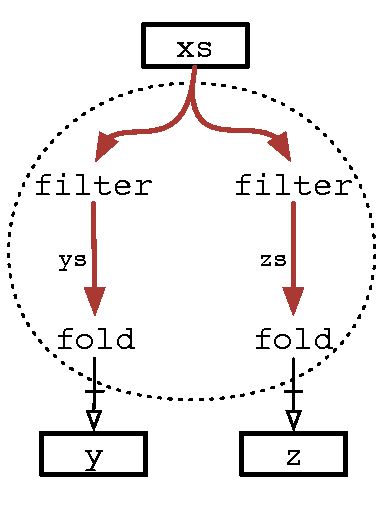
\includegraphics[scale=0.7]{copy/03-body/clustering/figures/ex4-concestors.pdf}
\end{center}
\end{minipage}
\caption{Program \Hs/sumPartition/ with clustering diagram}
\label{clustering:f:concestors}
\end{figure}

\begin{listing-c}[float,label=figs/clustering/sumPartition-c,caption=Unfused imperative implementation of \Hs/sumPartition/ with colour-coded iteration sizes]
void sumPartition(int* xs, size_t xs_length, int* out_y, int* out_z)
{
    // ys = filter ($>0$) xs
    int* ys = malloc(sizeof(int) * xs_length);
    size_t ys_length = 0;
    for (size_t i = 0; %\colorbox{green!10}{\tt{i != xs\_length}}%; ++i) {
        if (xs[i] > 0) ys[ys_length++] = xs[i];
    }

    // zs = filter ($<0$) xs
    int* zs = malloc(sizeof(int) * xs_length);
    size_t zs_length = 0;
    for (size_t i = 0; %\colorbox{green!10}{\tt{i != xs\_length}}%; ++i) {
        if (xs[i] < 0) zs[zs_length++] = xs[i];
    }

    // y = fold (+) 0 ys
    int y = 0;
    for (size_t i = 0; %\colorbox{purple!10}{\tt{i != ys\_length}}%; ++i) {
        y += ys[i];
    }
    *out_y = y;

    // z = fold (+) 0 zs
    int z = 0;
    for (size_t i = 0; %\colorbox{blue!10}{\tt{i != zs\_length}}%; ++i) {
        z += zs[i];
    }
    *out_z = z;

    free(ys);
    free(zs);
}
\end{listing-c}
\begin{listing-c}[float,label=figs/clustering/sumPartition-c-part,caption=Partially fused imperative implementation of \Hs/sumPartition/ with colour-coded iteration sizes]
void filter2(int* xs, size_t xs_length, int* out_y, int* out_z)
{
    // ys = filter ($>0$)  xs
    // y  = fold   (+) 0   ys
    int y = 0;
    for (size_t i = 0; %\colorbox{green!10}{\tt{i != xs\_length}}%; ++i) {
        if (xs[i] > 0) y += xs[i];
    }
    *out_y = y;

    // zs = filter ($<0$)  xs
    // z  = fold   (+) 0   zs
    int z = 0;
    for (size_t i = 0; %\colorbox{green!10}{\tt{i != xs\_length}}%; ++i) {
        if (xs[i] < 0) z += xs[i];
    }
    *out_z = z;
}
\end{listing-c}

We use the ancestor transducers to determine whether two combinators of different iteration sizes may be fused together.
\Cref{clustering:f:concestors} shows the \Hs/sumPartition/ example, which performs two filters over the same array, and computes the sum of each filter's output array.
The unfused imperative version, shown in \cref{figs/clustering/sumPartition-c}, performs each operation as a separate loop.
The last two loops compute the sums.
If we look at these two loops in isolation, the relationship between the two loop iteration sizes \Hs/ys_length/ and \Hs/zs_length/ is unknown, and it is not possible to fuse the two loops together without introducing excessively complicated control-flow.

The relationship between the two loop iteration sizes becomes clear when we consider each sum's parent transducer, which for the \Hs/y/ sum is the filter that produces \Hs/ys/, and for the \Hs/z/ sum is the filter that produces \Hs/zs/.
\Cref{figs/clustering/sumPartition-c-part} shows a partially fused imperative version, where each sum is fused with its parent transducer.
In this partially fused version, the two sums are still computed in separate loops, but both loops use the same iteration size.
Fusing these two loops together is trivial.

The key insight from this example is that two combinators of different iteration sizes may be fused together if each combinator is fused with its parent transducer, and the two parent transducers are also fused together.
If the two parent transducers also have different iteration sizes, their respective parent transducers must also be fused together.
In this case, we skip the parent transducers, and look directly at the closest pair of ancestor transducers with the same iteration size as each other.


\begin{figure}
% \begin{tabbing}
% MMMM \= M \= M \= M \= \kill
% $parents$ \> $:$ \> $binds \to name \to name \to \{name \times name\}$ \\
% $parents(bs, a, b)$ \\
%         \> $|$ \> $\iiter_{\Gamma,C}(bs(a)) == \iiter_{\Gamma,C}(bs(b))$ \\
%         \>     \>                      \> $=$ \> $\{(a, b)\}$ \\
%         \> $|$ \> otherwise            \\
%         \>     \>                      \> $=$    \> $\{ parents(bs, a', b) ~|~ a' \in trans(bs, a) \} $      \\
%         \>     \>                      \> $\cup$ \> $\{ parents(bs, a, b') ~|~ b' \in trans(bs, b) \} $  \\
% \end{tabbing}
% changed to return optional single closest parents:
%
\begin{tabbing}
MMMM \= M \= M \= M \= MMMM \= M \= \kill
$\concestors$ \> $:$ \> $\{\bind\} \to \name \to \name \to (\name \times \name)_\bot$ \\
$\concestors(bs, a, b)$ \\
        \> $|$ \> $(p_a,p_b,d) \in \concestors'(bs,a,b)$ \\
        \>     \>                      \> $=$ \> $\{(a, b)\}$ \\
        \> $|$ \> otherwise \\
        \>     \>                      \> $=$    \> $\bot$ \\
\\
$\concestors'$ \> $:$ \> $\{\bind\} \to \name \to \name \to (\name \times \name \times \mathbb{N})_\bot$ \\
$\concestors'(bs, a, b)$ \\
        \> $|$ \> $\iiter_{\Gamma,C}(bs(a)) == \iiter_{\Gamma,C}(bs(b))$ \\
        \>     \>                      \> $=$ \> $\{(a, b, 0)\}$ \\
        \> $|$ \> $a' \in \trans(bs,a),~ p_a \in \concestors'(bs,a',b)$ \\
        \> $,$ \> $b' \in \trans(bs,b),~ p_b \in \concestors'(bs,a,b')$ \\
        \>     \>                      \> $=$ \> $\mi{increment}(\mi{closest}(p_a, p_b))$ \\
        \> $|$ \> $a' \in \trans(bs,a),~ p_a \in \concestors'(bs,a',b)$ \\
        \>     \>                      \> $=$ \> $\mi{increment}(p_a)$ \\
        \> $|$ \> $b' \in \trans(bs,b),~ p_b \in \concestors'(bs,a,b')$ \\
        \>     \>                      \> $=$ \> $\mi{increment}(p_b)$ \\
        \> $|$ \> otherwise            \\
        \>     \>                      \> $=$    \> $\bot$
\\
\\
$\mi{closest}$ \> $:$ \> $(\name \times \name \times \mathbb{N}) \to (\name \times \name \times \mathbb{N}) \to (\name \times \name \times \mathbb{N})$ \\
$\mi{closest}((l_a,l_b,l_d), (r_a,r_b,r_d))$ \\
        \> $|$ \> $l_d \le r_d$ \> \> \> $=$ \> $(l_a,l_b,l_d)$ \\
        \> $|$ \> otherwise     \> \> \> $=$ \> $(r_a,r_b,r_d)$ \\
\\
$\mi{increment} :$ \> \> $(\name \times \name \times \mathbb{N}) \to (\name \times \name \times \mathbb{N})$ \\
$\mi{increment}((a,b,d)) = (a,b,d+1)$ \\
\end{tabbing}

\caption{Finding the compatible concestors, or most recent common ancestors with the same iteration size}
\label{fig:clustering:concestors}
\end{figure}

\Cref{fig:clustering:concestors} defines the $\concestors$ function, which finds the pair of most recent common ancestor transducers such that both ancestors have the same iteration size.
In the field of biological systematics, the term \emph{concestor} is defined as the most recent common ancestor; here, we define the \emph{compatible concestors} of a transducer to be the pair of most recent common ancestors with the same iteration size.
In the definition of the $\concestors$ function, we use the syntax $(name \times name)_\bot$ to denote an optional pair of names.
Two combinators $a$ and $b$ of different iteration size may be fused together only if they have compatible concestors $(c, d) \in \concestors(a,b)$, and the combinators and their compatible concestors are also fused together.
That is, in order for $a$ and $b$ to be fused together, $c$ and $d$ must be fused, $a$ and $c$ must be fused, and $d$ and $b$ must be fused.
If the two combinators $a$ and $b$ have the same iteration size, then the two compatible concestors will be the combinators themselves, and the above requirements for fusing different sized combinators are trivially satisfied, since a combinator is always fused with itself.

Still in \cref{fig:clustering:concestors}, the definition of $\concestors'$ returns the pair of compatible concestors as well as the distance, determined by counting how many other ancestor transducers there are between the combinator and the compatible concestors.
The $\mi{closest}$ function compares the distances of two pairs of compatible concestors and chooses the closest pair.
The $\mi{increment}$ function increases the distance by one.

The $\trans$ function returns only the direct parent transducer, but a single combinator can have multiple ancestor transducers.
For a pair of combinators with multiple ancestor transducers, there may be multiple compatible common ancestors, but there can only be one pair of \emph{most recent} compatible common ancestors (compatible concestors), because of the tree structure of ancestor transducers.
In general, a pair of differently-sized combinators could be fused together if \emph{any} pair of compatible common ancestors are fused together with the combinators.
Because fusing the combinators with any pair of compatible common ancestors requires fusing with the compatible concestors as well, it is sufficient to require the pair of combinators to be fused with just the compatible concestors.

% Because each node has at most one transducer, and each transducer introduces a unique output size, the graph of ancestors forms a tree rather than a directed acyclic graph.
% A pair of nodes can have at most one most recent compatible common ancestor transducers, because each node has at most one transducer, and each transducer introduces a unique output size.
% This means that the ancestors are defined as a tree, rather than a directed acyclic graph, and each pair of nodes has a single common ancestor transducer.
% Two nodes cannot have the same iteration size if they have different parent transducers.
% A pair of nodes can have at most one pair of compatible concestors because each transducer has a unique output size.
% This means that, for two ancestor transducers to have the same iteration size, 

% Intuitively, a pair of nodes can have at most one pair of compatible concestors, because the transducers form a total ordering, and 
% The \emph{sole transducers} lemma ensures that a pair of nodes can have at most one pair of compatible concestors.
% If two nodes have a pair compatible concestors, it is unique, thanks to the \emph{sole transducers} lemma.
% To fuse a combinator with a particular ancestor, we must also fuse the combinator with all the nodes in the path between the combinator and its ancestor.
% In the definition of $\concestors$, we find the closest ancestors because it allows the most fusion; finding the furthest ancestors would be more restrictive, as it would also require fusing the inputs with any other ancestor transducers between the input combinators and the furthest ancestors.

The \Hs/normalize2/ example from earlier is repeated in \cref{figs/clustering/normalize2-sizeinf}.
In this example, \Hs@sum1@ consumes the input \Hs/xs/, while \Hs@sum2@ consumes the output of the filter \Hs/gts/, which in turn consumes the input \Hs/xs/.
The two folds have different iteration sizes, and their compatible concestors are $\concestors(\Hs@sum1@, \Hs@sum2@) = (\Hs@sum1@, \Hs@gts@)$.
The compatible concestors \Hs/sum1/ and \Hs/gts/ both consume the input \Hs/xs/ and have the same iteration size.
In order for \Hs@sum1@ and \Hs@sum2@ to be fused together, we require that: \Hs@sum1@ and \Hs@gts@ are fused together; \Hs@sum1@ and \Hs@sum1@ are fused together, which is trivial as fusion is reflexive;  and \Hs@gts@ and \Hs@sum2@ are fused together.

\begin{haskell}[float,label=figs/clustering/normalize2-sizeinf,caption=Normalize2 function]
normalize2 :: Array Int -> (Array Int, Array Int)
normalize2 xs
 = let sum1 = fold   (+)  0   xs
       gts  = filter (>   0)  xs
       sum2 = fold   (+)  0   gts
       ys1  = map    (/ sum1) xs
       ys2  = map    (/ sum2) xs
   in (ys1, ys2)
\end{haskell}


%!TEX root = ../Main.tex

\begin{figure}
\begin{center}
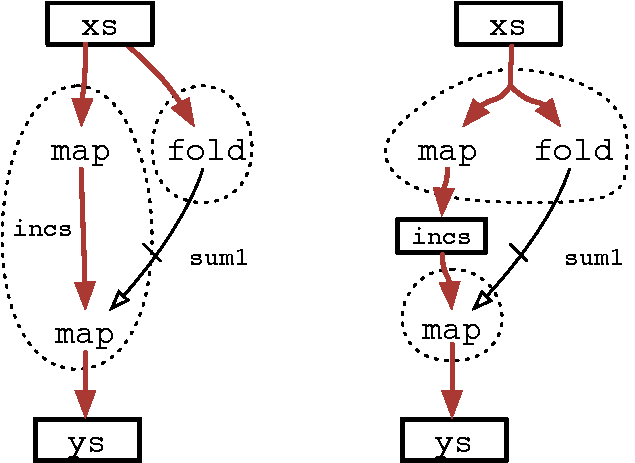
\includegraphics[scale=0.5]{copy/03-body/clustering/figures/ex2-normalizeInc.pdf}
\end{center}
\caption{Possible clusterings for \Hs/normalizeInc/}
\label{clustering:f:normalizeInc}
\end{figure}


% -----------------------------------------------------------------------------
\section{Integer linear programming}
\label{clustering:s:ILP}
It is usually possible to cluster a program graph in multiple ways.
For example, consider the following simple function:
\begin{haskell}
normalizeInc :: Array Int -> Array Int
normalizeInc xs
 = let incs = map  (+1)     us
       sum1 = fold (+) 0    us
       ys   = map  (/ sum1) incs
   in  ys
\end{haskell}

Two possible clusterings are shown in \cref{clustering:f:normalizeInc}.
One option is to compute \Hs@sum1@ first and fuse the computation of \Hs@incs@ and \Hs@ys@.
Another option is to fuse the computation of \Hs@incs@ and \Hs@sum1@ into a single loop, then compute \Hs@ys@ separately.
A third option (not shown) is to compute all results separately, and not perform any fusion. 

Which option is better?
On current hardware, we generally expect the cost of memory access to dominate runtime.
The first clustering in \cref{clustering:f:normalizeInc} requires two reads from array \Hs@xs@ and one write to array \Hs@ys@.
The second clustering requires a single fused read from \Hs@xs@, one write to \Hs@incs@, a read back from \Hs@incs@ and a final write to \Hs@ys@.
From the size constraints of the program, we know that all intermediate arrays have the same size, so we expect the first clustering will peform better as it only needs three array accesses instead of four. 

For small programs such as \Hs@normalizeInc@, it is possible to naively enumerate all possible clusterings, select just those that are \emph{valid} with respect to fusion preventing edges, and choose the one that maximises a cost metric such as the number of array accesses needed.
However, as the program size increases the number of possible clusterings becomes too large to naively enumerate.
For example, \citet{pouchet2010combined,pouchet2011polyhedral} present a fusion system using the polyhedral model and report that some simple numeric programs have over 40,000 possible clusterings, with one particular example having $10^{12}$ clusterings.

To deal with the combinatorial explosion in the number of potential clusterings, we instead use an integer linear programming (ILP) formulation.
ILP problems are defined as a set of variables, an objective linear function and a set of linear constraints.
The integer linear solver finds an assignment to the variables that minimises the objective function, while satisfying all constraints.
For the clustering problem, we express our constraints regarding fusion preventing edges as linear constraints on the ILP variables, then use the objective function to encode our cost metric.
This general approach was first fully described by \citet{megiddo1998optimal}; the main contribution of this chapter is to extend their formulation to work with size-changing operators such as \Hs@filter@. 


% -----------------------------------------------------------------------------
\subsection{Dependency graphs}
A dependency graph represents the data dependencies of the program to be fused, and we use it as an intermediate stage when producing linear constraints for the ILP problem. The dependency graph contains enough information to determine the possible clusterings of the input program, while abstracting away from the exact operators used to compute each intermediate array. The rules for producing dependency graphs are shown in \cref{clustering:f:DependencyGraph}.

\begin{figure}
\begin{tabbing}
MMMM       \= MM  \= \kill
$V$ \> @::=@ \> $\{(\name \times T)\}$ \\
$E$ \> @::=@ \> $\{(\name \times \name \times E_T)\}$ \\
$E_T$ \> @::=@ \> $\fusible ~|~ \fusionpreventing$ \\
\\
$\nodes$     \> @  :@ \> $\program \to V$                          \\
$\nodes(bs)$ \> $~~= \{(\name(b), \iiter_{\Gamma,C}(b)) ~|~ b \in bs\}$
\\
\\
$\edges$     \> @  :@ \> $\program \to E$                          \\
$\edges(bs)$ \> $~~= \bigcup_{b \in bs} \edge(bs, b)$
\\
\\
MM             \= M \= $\Hs@gather@~$ \= $\data~\indices$ \= \kill
$\edge$      \> ~@:@ \> $\{\bind\} \times \bind \to E$ \\
$\edge(bs, \out = b)$ \\
   \> $~|$ \> $\Hs@fold@$ \> $f~in$ \> $\gets b$ \\
   \> $~|$ \> $\Hs@map@$ \> $f~in$ \> $\gets b$ \\
   \> $~|$ \> $\Hs@filter@$ \> $f~in$ \> $\gets b$ \\
    \> $=$    \> $\{\inedge(bs,\out,s) ~|~ s \in \fv(f)\} \cup \{\inedge(bs, \out, in) \}$
\\[1ex]
% $\edge(bs, \out = \Hs@map@~f~in)$  \\
%     \> $=$    \> $\{\inedge(bs,\out,s) ~|~ s \in \fv(f)\} \cup \{\inedge(bs, \out, in) \}$
% \\
% $\edge(bs, \out = \Hs@filter@~f~in)$ \\
%     \> $=$    \> $\{\inedge(bs,\out,s) ~|~ s \in \fv(f)\} \cup \{\inedge(bs, \out, in) \}$
% \\
   \> $~|$ \> $\Hs@gather@~\data~\indices$ \> \> $\gets b$ \\
% $\edge(bs, \out = \Hs@gather@~data~indices)$ \\
    \> $=$    \> $\{(\out,\data, \fusionpreventing) \} \cup \{\inedge(bs, \out, \indices) \}$      
\\[1ex]
   \> $~|$ \> $\Hs@cross@~a~b$ \> \> $\gets b$ \\
% $\edge(bs, \out = \Hs@cross@~a~b)$ \\
    \> $=$    \> $\{\inedge(bs, \out, a) \}           \cup      \{(\out, b, \fusionpreventing) \}$
\\[1ex]
   \> $~|$ \> $\Hs@external@~ins$ \> \> $\gets b$ \\
% $\edge(bs, \outs = \Hs@external@~ins)$  \\
    \> $=$    \> $\{(o,i, \fusionpreventing) ~|~ o \in \out,~ i \in ins \}$
\\
\\
$\inedge$ @:@ $\{\bind\} \times \name \times \name \to (\name \times \name \times E_T)$
\\
$\inedge(bs,to,\from)$ \\
    \> $~|$ \> $(\from = \Hs@fold@~f~s) \in bs$     \\
    \> $=$ \> $(to, \from, \fusionpreventing)$
\\[1ex]
    \> $~|$ \> $(\outs = \Hs@external@ \ldots) \in bs     \wedge \from \in \outs$     \\
    \> $=$ \> $(to, \outs, \fusionpreventing)$
\\[1ex]
    \> $~|$ \> $otherwise$                      \\
    \> $=$ \> $(to, \from, \fusible)$
\end{tabbing}

\caption{Dependency Graphs from Programs}
\label{clustering:f:DependencyGraph}
\end{figure}



Each binding in the source program becomes a node in the dependency graph.
For each intermediate variable, we add a directed edge from the binding that produces a value to all bindings that consume it.
Each edge is also marked as either \emph{fusible} or \emph{fusion-preventing}.
Fusion-preventing edges are used when the producer must finish its execution before the consumer node can start.
For example, a \Hs@fold@ operation must complete execution before it can produce the scalar value needed by its consumers.
Conversely, the \Hs@map@ operation produces an output value for each value it consumes, so is marked as fusible. 

The \Hs@gather@ operation is a hybrid: it takes an indices array and an elements array, and for each element in the indices array returns the corresponding data element. This means that gather can be fused with the operation that produces its indices, but not the operation that produces its elements --- because those are accessed in a random-access manner. 

% Each node may simply be the name of its output binding (or bindings, in the case of \Hs@external@); as we require names to only be bound once, this is assured to be unique. Creating edges between these nodes is simply when one binding references an earlier one. The only complication is designating edges as \emph{fusible} or \emph{fusion-preventing}.



% -----------------------------------------------------------------------------
\subsection{ILP Variables}
After generating the dependency graph, the next step is to produce a set of linear constraints from this graph.
The variables involved in these constraints are split into three groups, labelled $x$, $\pi$, and $c$.
The first group of variables, $x$, is parameterised by a pair of input nodes:

\begin{tabbing}
M   \= MM \= MMMMMMM \= MM \= \kill
$x$   \> @:@  \> $node \times node$ \> $\to$ \> $\mathbb{B}$
\end{tabbing}

For each pair of nodes with indices $i$ and $j$, we use a boolean variable $x_{i,j}$, which indicates whether those two nodes are fused.
We use $x_{i,j} = 0$ when the nodes are fused and $x_{i,j} = 1$ when they are not.
Using $0$ for the fused case means that the objective function can be a weighted function of the $x_{i,j}$ variables, and minimizing it tends to increase the number of nodes that are fused.
The values of these variables are used to construct the final clustering, such that $\forall i,j.\ x_{i,j} = 0 \iff \mathit{cluster}(i) = \mathit{cluster}(j)$.

The second group of variables, $\pi$, is parameterised by a single node:

\begin{tabbing}
M   \= MM \= MMMMMMM \= MM \= \kill
$\pi$ \> @:@  \> $node$             \> $\to$ \> $\mathbb{R}$
\end{tabbing}

This group of variables is used to ensure that the clustering is acyclic.
An acyclic clustering is necessary to be able to execute the resulting clustering: we need to ensure that for each node in the graph, the dependencies of that node can be executed before the node itself.
For each node $i$, we associate a real $\pi_i$ such that every node $j$ that depends on $i$ we have $\pi_j > \pi_i$.
Our linear constraints will ensure that if two nodes are fused into the same cluster then their $\pi$ values will be identical --- though nodes in different clusters can also have the same $\pi$ value.
Here is an example of a cyclic clustering, with the cluster (C1) or (C2) specified on the right:
\begin{haskell}
  cycle xs  = let ys  = map (+1) xs     -- (C1)
                  sum = fold ys         -- (C2)
                  zs  = map (+sum) ys   -- (C1)
              in  zs
\end{haskell}

There is no fusion-preventing edge directly between the \Hs@xs@ and \Hs@zs@ bindings, but there is a fusion-preventing edge between \Hs@sum@ and \Hs@zs@.
If the \Hs@xs@ and \Hs@zs@ bindings were in the same cluster (C1) and \Hs@sum@ was in cluster (C2), there would be a dependency cycle between (C1) and (C2), and neither could be executed before the other.

The third, and final, group of variables is parameterised by a single node:
\begin{tabbing}
M   \= MM \= MMMMMMM \= MM \= \kill
$c$   \> @:@  \> $node$             \> $\to$ \> $\mathbb{B}$
\end{tabbing}

This final group of variables is used to help define the cost model encoded by the objective function.
As in \citet{darte2002contraction}, each node is assigned a variable $c_i$ that indicates whether the array the associated binding produces is \emph{fully contracted}.
When an array is fully contracted, it means that all consumers of that array are fused into the same cluster, so we have $c_i = 0 \iff (\forall (i',j) \in E.\ i = i' \implies x_{i,j} = 0)$.
In the final program, each successive element of a fully contracted array can be stored in a scalar register, rather than requiring an array register or memory storage. 


% -----------------------------------------------------------------------------
\subsection{Linear Constraints}
\label{clustering:s:LinearConstraints}
The constraints we place on the ILP variables are split into four groups: constraints that ensure the clustering is acyclic; constraints that encode fusion preventing edges; constraints on nodes with different iteration sizes, and constraints involving array contraction. 

% Before showing the optimised version with certain constraints removed (\cref{clustering:s:OptimisedConstraints}), this simpler, unoptimised version is shown. The only difference is that fewer constraints and variables are required in the optimised version, but both versions give the same clustering. This unoptimised version generates clustering constraints and variables for every pair of nodes, regardless of whether they may, in fact, be fused together. Later, we show that certain constraints and variables can be removed when there is a fusion-preventing edge between two nodes.


% -------------------------------------
\paragraph{Acyclic and precedence-preserving} The first group of constraints ensures that the clustering is acyclic:
\begin{tabbing}
MM  \= MMMx \= M \= MMM \= M \= MMMM \= \kill
    \> ~~~~~~~ $x_{i,j}$ \> $\le$ \> $\pi_j - \pi_i$ \> $\le$ \> $N \cdot x_{i,j}$ 
    \>             (with an edge from $i$ to $j$)            \\
    \> $-N \cdot  x_{i,j}$  \> $\le$ \> $\pi_j - \pi_i$ \> $\le$ \> $N \cdot x_{i,j}$ 
    \>             (with no edge from $i$ to $j$)
\end{tabbing}

As per Megiddo~\cite{megiddo1998optimal} the form of these constraints is determined by whether there is an dependency between nodes $i$ and $j$. The $N$ value is set to the total number of nodes in the graph.

If there is an edge from node $i$ to $j$ we use the first constraint form shown above. If the two nodes are fused into the same cluster then we have $x_{i,j} = 0$. In this case the constraint simplifies to $0 \le \pi_j - \pi_i \le 0$, which forces $\pi_i = \pi_j$. If the two nodes are in \emph{different} clusters then the constraint instead simplifies to $1 \le \pi_j - \pi_i \le N$. This means that the difference between the two $\pi$s must be at least 1, and less than $N$. Since there are $N$ nodes, the maximum difference between any two $\pi$s would be at most $N$, so the upper bound of $N$ is large enough to be safely ignored. This means the constraint can roughly be translated to $\pi_i < \pi_j$, which enforces the acyclicity constraint.

If instead there is no edge from node $i$ to $j$ then we use the second constraint form above. As before, if the two nodes are fused into the same cluster then we have $x_{i,j} = 0$, which forces $\pi_i = \pi_j$. If the nodes are in different clusters then the constraint simplifies to $-N \le \pi_j - \pi_i \le N$, which effectively puts no constraint on the $\pi$ values.


% -------------------------------------
\paragraph{Fusion-preventing edges} As per Megiddo~\cite{megiddo1998optimal}, if there is a fusion preventing edge between two nodes we add a constraint to ensure the nodes will be placed in different clusters.
\begin{tabbing}
MMM     \= MMM \= M  \= MMM \= M \= MMM \= \kill
        \> $x_{i,j}$ \> $=$ \> $1$ \>   \> \\
        \> (for fusion-preventing edges from $i$ to $j$) 
\end{tabbing}

When combined with the precedence-preserving constraints earlier, setting $x_{i,j} = 1$ also forces $\pi_i < \pi_j$. 


% -------------------------------------
\paragraph{Fusion between different iteration sizes} This group of constraints restricts which nodes can be placed in the same cluster based on their iteration size. The group has three parts. 
Firstly, either of the two nodes connected by an edge have an unknown ($\bot$) iteration size then they cannot be fused and we set $x_{i,j} = 1$:
\begin{tabbing}
MMM     \= MMM \= M \= MMM \= M \= MMM \= \kill
        \> $x_{i,j}$   \> $=$   \> $1$          \>       \>     \\
        \> (if $\iiter_{\Gamma,C}(i) = \bot 
                ~\vee~ \iiter_{\Gamma,C}(j) = \bot$)
\end{tabbing}

Secondly, if the two nodes have different iteration sizes and no common parent then they also cannot be fused and we set $x_{i,j} = 1$:
\begin{tabbing}
MMM     \= MMM \= M \= MMM \= M \= MMM \= \kill
        \> $x_{i,j}$   \> $=$   \> $1$          \>       \>     \\
        \> (if $\iiter_{\Gamma,C}(i) \not= \iiter_{\Gamma,C}(j) 
                ~\wedge~ parents(i,j) = \emptyset$)
\end{tabbing}

Finally, if the two nodes had different iteration sizes but \emph{do} have parent transducers of the same size, then the two nodes can be fused if they are fused with their respective parents, and the parents themselves are fused:
\begin{tabbing}
MMM     \= MMM \= M \= MMM \= M \= MMM \= \kill
        \> $x_{a,A}$   \> $\le$ \> $x_{a,b}$    \>       \>     \\
        \> $x_{b,B}$   \> $\le$ \> $x_{a,b}$    \>       \>     \\
        \> $x_{A,B}$   \> $\le$ \> $x_{a,b}$    \>       \>     \\
        \> (if $\iiter_{\Gamma,C}(a) \not= \iiter_{\Gamma,C}(b) 
                ~\wedge~ parents(a,b) = \{(A,B)\}$)
\end{tabbing}

This last part is the main difference to existing ILP solutions: we allow nodes with different iteration sizes to be fused when their parent transducers are fused. The actual constraints encode a ``no more fused than'' relationship. For example $x_{a,A} \le x_{a,b}$ means that nodes $a$ and $b$ can be no more fused than nodes $a$ and $A$. 

As a simple example, consider fusing an operation on filtered data with its generating filter:
\begin{haskell}
    sum1 = fold (+) 0  xs
    gts  = filter (>0) xs
    sum2 = fold (+) 0  gts
\end{haskell}

Here $sum1$ and $sum2$ have different iteration sizes and we have that $parents(sum1, sum2) = \{(sum1, gts)\}$. This means that $sum1$ and $sum2$ may only be fused if $sum1$ is fused with $sum1$ (trivial), $sum2$ is fused with $gts$, and $sum1$ is fused with $gts$.

% Here, $parents(gts,sum2) = \{gts, gts\}$. This generates spurious, but still valid, constraints that $gts$ must be fused with $gts$ and $gts$ must be fused with $sum2$, in order for $gts$ and $sum2$ to be fused together. While these constraints are unnecessary in this case, they are harmless.

% While it may seem like these constraints should be implied by transitivity of clustering, all clustering variables are used for the objective function.


% -------------------------------------
\paragraph{Array contraction} The final group gives meaning to the $c$ variables, which represent whether an array is fully contracted:
\begin{tabbing}
MMM     \= MMM \= M \= MMM \= M \= MMM \= \kill
        \> $x_{i,j}$    \> $\le$ \> $c_i$  \> \> \\
        \> (for all edges from i)
\end{tabbing}

Recall that an array is fully contracted when all of the consumers are fused with the nodes that produces it, which means that the array does not need to be fully materialized in memory. As per Darte's work on array contraction~\cite{darte2002contraction}, we define a variable $c_i$ for each array, and the constraint above ensures that $c_i = 0$ only if $\forall (i',j) \in E.\ i = i' \implies x_{i,j} = 0$. By minimizing $c_i$ in the objective function, we favor solutions that reduce the number of intermediate arrays.


% -----------------------------------------------------------------------------
\subsection{Objective Function}
\label{clustering:s:ObjectiveFunction}
The objective function defines the cost model of the program, and the ILP solver will find the clustering that minimizes this function while satisfying the constraints defined in the previous section. The cost model we use in this paper has three components:
\begin{itemize}
\item
the number of array reads and writes --- an abstraction of the amount of memory bandwidth needed by the program; 
\item
the number of intermediate arrays --- an abstraction of the amount of intermediate memory needed; 
\item
the number of distinct clusters --- an abstraction of the cost of loop management instructions, which maintain loop counters and the like.
\end{itemize}

The three components of the cost model are a heuristic abstraction of the true cost of executing the program on current hardware. They are ranked in order of importance --- so we prefer to minimize the number of array reads and writes over the number of intermediate arrays, and to minimize the number of intermediate arrays over the number of clusters. However, minimizing one component does not necessarily minimize any other. For example, as the fused program executes multiple array operations at the same time, in some cases the clustering that requires the least number of array reads and writes uses more intermediate arrays than strictly necessary.

We encode the ordering of the components of the cost model as different weights in the objective function. First, note that if the program graph contains $N$ combinators (nodes) then there are at most $N$ opportunities for fusion. We then encode the relative cost of loop overhead as weight $1$, the cost of an intermediate array as weight $N$, and the cost of an array read or write as weight $N^2$. This ensures that no amount of loop overhead reduction can outweigh the benefit of removing an intermediate array, and likewise no number of removed intermediate arrays can outweigh a reduction in the number of array reads or writes. The integer linear program including the objective function is as follows:
\begin{tabbing}
MMMMM   \= MMMM \= M \= \kill
Minimise   \>     $\Sigma_{(i,j) \in E} W_{i,j} \cdot x_{i,j}$   
                        ~~ (memory traffic and loop overhead)
\\ ~~~~~~~~~~~~~ $+$ \> $\Sigma_{i \in V} N \cdot c_i$
                        ~~~~~~~~~~~~ (removing intermediate arrays)
\\[1ex]
   Subject to  \> \ldots ~ constraints from \cref{clustering:s:LinearConstraints} ~ \ldots 
\\ Where   \> $W_{i,j} = N^2$ \> $~|$ \> $(i,j) \in E $         
\\         \> \> \> (fusing $i$ and $j$ will reduce memory traffic)         
\\         \> $W_{i,j} = N^2$ \> $~|$ \> $\exists k. (k,i) \in E \wedge (k,j) \in E $     
\\         \> \> \> ($i$ and $j$ share an input array)
\\         \> $W_{i,j} = 1$   \> $~|$ \> $\Hs@otherwise@$
\\         \> \> \> (the only benefit is loop overhead)
\\         \> $N = |V|$
\end{tabbing}

% However, these benefits cannot be considered in isolation; for example, fusing two loops to reduce loop overhead may remove potential fusion opportunities that reduce memory traffic. When operating on large arrays that do not fit in cache, memory traffic dominates execution time. An excessive number of intermediate arrays can also cause issues if all are live in memory at once, potentially leading to \emph{thrashing}. The benefits of removing loop overhead are least of all; it should be performed if possible, but must never remove opportunities for other fusion.



% -----------------------------------------------------------------------------
\subsection{Fusion-preventing Path Optimisation}
\label{clustering:s:OptimisedConstraints}
The integer linear program defined in the previous section includes more constraints than strictly necessary to define the valid clusterings. If two nodes have a path between them which includes a fusion preventing edge, then we know up front that they must be placed in different clusters. The following function $possible(a,b)$ determines whether there is any possibility that the two nodes $a$ and $b$ can be fused. Similarly the function $possible'(a, b)$ checks whether there is any possibility that the parents of $a$ and $b$ may be fused.
%
\begin{tabbing}
MMMM \= M \=     \= MMMMMMMMMMMM    \=  \kill
$possible$ \> $:$     \> $name \times name \to \mathbb{B}$      \\
MMMMMMx        \= M    \= \kill
$possible(a,b)$   
        \> $=$  \>$\forall p \in path(a,b) \cup path(b,a).\ \fusionpreventing \not\in p$
\\[1ex]
MMMM \= M \=     \= MMMMMMMMMMMM    \=  \kill
$possible'$     \> $:$ \> $name \times name \to \mathbb{B}$      \\
MMMMMMx        \= M    \= \kill
$possible'(a,b)$ 
        \> $=$   \>$\exists A, B.\  parents(a,b) = \{A,B\} \wedge possible(a,b)$ \\
        \> $\wedge$ \> $possible(A,a) \wedge possible(B,b) \wedge possible(A,B)$
\end{tabbing}

With $possible$ and $possible'$ defined, we refine our formulation to only generate constraints between two nodes if there is a chance they may be fused together. Doing this reduces the total number of constraints, and makes the job of the ILP solver easier. The final formulation of the integer linear program follows.
%
\begin{tabbing}
MMMMM   \= MMMM \= M \= MMMM \= M \= MMMM \= \kill
Minimise   \> $\Sigma_{(i,j) \in E} W_{i,j} \cdot x_{i,j} + \Sigma_{i \in V} N \cdot c_i$  \\
           \> (if $possible(i,j)$)         
\\[0.5ex]
Subject to \> $-N \cdot x_{i,j}$ \> $\le$ \> $\pi_j - \pi_i$ \> $\le$ \> $N \cdot x_{i,j}$ \\
           \> (if $possible(i,j) \wedge (i,j) \not\in E \wedge (j,i) \not\in E$)            
\\[0.5ex]
           \>    $x_{i,j}$ \> $\le$ \> $\pi_j - \pi_i$ \> $\le$ \> $N \cdot x_{i,j}$ \\
           \> (if $possible(i,j) \wedge (i,j,\fusible) \in E$)     
\\[0.5ex]
           \>             \>       \> $\pi_i < \pi_j$ \>       \>            \\
           \> (if $(i,j,\fusionpreventing) \in E$)    
\\[0.5ex]
           \> $x_{i,j}$    \> $\le$ \> $c_i$           \>       \>            \\
           \> (if $(i,j, \fusible) \in E$) \\
           \> $c_{i }$    \> $ = $ \> $ 1 $           \>       \>            \\
           \> (if $(i,j, \fusionpreventing) \in E$)
\\[0.5ex]
           \> $x_{i,j}$    \> $=$   \> $1$             \>       \>            \\
           \> (if $\bot \in \{\iiter_{\Gamma,C}(i), \iiter_{\Gamma,C}(j)\}$)  
\\[0.5ex]
           \> $x_{i',i}$   \> $\le$ \> $x_{i,j}$        \>       \>            \\
           \> $x_{j',j}$   \> $\le$ \> $x_{i,j}$        \>       \>            \\
           \> $x_{i',j'}$   \> $\le$ \> $x_{i,j}$        \>       \>            \\
           \> (if $\iiter_{\Gamma,C}(i) \not= \iiter_{\Gamma,C}(j) \wedge possible'(i,j)$ \\
           \> \> $\wedge~parents(i,j) = \{(i',j')\}$) 
\\[0.5ex]
           \> $x_{i,j}$    \> $=$   \> $1$             \>       \>            \\
           \> (if $\iiter_{\Gamma,C}(i) \not= \iiter_{\Gamma,C}(j) \wedge \neg possible'(i,j)$) 
\\[0.5ex]
MMMMM   \= MMMM \= M \= \kill
Where      \> $W_{ij} = N^2$ \> $~|$ \> $(i,j) \in E $         \\
           \> \> \> (fusing $i$ and $j$ will reduce memory traffic)         \\
           \> $W_{ij} = N^2$ \> $~|$ \> $\exists k. (k,i) \in E \wedge (k,j) \in E $     \\
           \> \> \> ($i$ and $j$ share an input array)                                         \\
           \> $W_{ij} = 1$   \> $~|$ \> $\Hs@otherwise@$                                                  \\
           \> \> \> (the only benefit is loop overhead)                                        
\\
           \> $N = |V|$
\end{tabbing}

% % !!!!!!!!!!!!!!!!!!!!!!!
% I commented the \input out in section/04-ILP.tex

\subsection{Proof}
To prove correctness of our linear program formulation, we need to prove two different things.
Firstly, the formulation's constraints must always be satisfiable; that is, there must exist a variable assignment that satisfies all constraints.
This is rather simple to show, but guarantees that the linear program will always give an answer.
The next thing to show is that any produced clustering is legal: if a variable assignment satisfies the constraints, then it is a valid and legal clustering.
This means that, not only do we get \emph{an} answer, we also get the \emph{right} answer.

%!TEX root = ../Main.tex
\subsubsection{Satisfiability}
For any program $p$, there exists a trivial clustering with no fusion at all.
We can use this as the variable assignment of $ilp(p)$.
For each pair of nodes $m,n \in p$, $x_{mn} = 1$ --- no fusion is possible.
For the $\pi$ variables, we must find a topographical ordering of the nodes in $p$, which is simple since we are assured it is a dag.

\TODO{Now, prove that this assignment actually satisfies the constraints.}


\subsubsection{Soundness}
For any program $p$ and variable asignment $v$, if $v$ satisfies the constraints for $ilp(p)$, the clustering denoted by $x_{ij}$ in $v$ is legal.

For a clustering to be legal, it must satisfy three constraints:
\begin{description}
\item[Acyclic]
after merging nodes of same cluster together, the resulting graph must be a dag
\item[Precedence preserving]
if there is an edge between two nodes $i$ and $j$, and they are not merged together, then we require $\pi_j > \pi_i$
\item[Fusion preventing]
likewise, if there is a fusion-preventing edge between two nodes $i$ and $j$, then we require $\pi_j > \pi_i$, which implies that they are not merged together
\item[Type constraint]
if two nodes $i$ and $j$ are in the same cluster, then $\tau_i = \tau_j$, or if $\tau_i$ is a subtype of $\tau_j$ (or $\tau_j$ is a subtype of $\tau_i$), then the \emph{generator} for $\tau_i$ (or $\tau_j$) must also be in the same cluster as $i$ and $j$.
    \\
    \TODO Actually, let us say $x_{ij} = 0 \implies check_{ij}$

\end{description}
where
\begin{tabbing}
MMMMM      \= M \= MMMMMMM \= MM \= \kill
$check$ \> @::@  \> $array \times array$ \> $\to$ \> $\mathbb{B}$ \\
MMMMM      \= M \= MMMMMM \= MM \= \kill
$check(i, j)$     \> $|$ \> $tau_i = tau_j$ \> $=$ \> $x_{i,j} = 0$                        \\
$check(i, j)$     \> $|$ \> $i' \in gen(i) $ \> $=$ \> $x_{i',j} = 0 \wedge x_{i,i'} = 0 \wedge check(i', j)$                        \\
$check(i, j)$     \> $|$ \> $j' \in gen(j) $ \> $=$ \> $x_{i,j'} = 0 \wedge x_{j,j'} = 0 \wedge check(i, j')$                        \\
$check(i, j)$     \> $|$ \> $tau_i \not= tau_j$\> $=$ \> $\bot$
\end{tabbing}









%!TEX root = ../Main.tex
\section{Benchmarks}
\label{clustering:s:Benchmarks}

\begin{table}
$$\begin{array}{c}

\begin{tabular}{lrrrrrrrr}
                & \multicolumn{2}{c}{Unfused}         & \multicolumn{2}{c}{Stream}
                & \multicolumn{2}{c}{Megiddo} &\multicolumn{2}{c}{\textbf{Ours}} \\
                & Time & Loops   & Time & Loops      & Time & Loops & Time & Loops   \\
\hline
Normalize2      & 1.88s & 5      & 1.64s & 4          & 1.82s & 3  & \textbf{1.59s} & \textbf{2}\\
Closest points  & 3.83s & 7      & 3.33s & 6          & 2.92s & 4  & \textbf{2.92s} & \textbf{4}\\
QuadTree        & 5.22s & 8      & 5.22s & 8          & 4.72s & 2  & \textbf{4.72s} & \textbf{2}\\
\end{tabular}

\end{array}$$
\caption{Benchmark results}
\label{clustering:f:BenchResults}
\end{table}

This section discusses three representative benchmarks, and gives the full ILP program of the first benchmark.
These benchmarks highlight the main differences between our fusion mechanism and related work.
The runtimes of each benchmark are summarized in \cref{clustering:f:BenchResults}.
We report times for: the unfused case, where each operator is assigned to its own cluster; the clustering implied by pull-based stream fusion~\cite{coutts2007stream}; the clustering chosen by Megiddo~\cite{megiddo1998optimal}; and the clustering chosen by our system. 

For each benchmark, we report the runtimes of hand-fused C code based on the clustering determined by each algorithm.
Although in a production implementation of clustering we would use the process fusion from \cref{chapter:process:processes} to fuse each cluster, we report on hand-fused C code to provide a fair comparison to related work.
As mentioned in~\citet{lippmeier2013data}, the current Haskell stream fusion mechanism introduces overhead in terms of a large number of duplicate loop counters, which increases register pressure unnecessarily.
Hand-fusing all code and compiling it with the same compiler (GCC) isolates the true cost of the various clusterings from low-level differences in code generation.

We have used both GLPK and CPLEX as external ILP solvers.
For small programs such as \Hs@normalizeInc@, both solvers produce solutions in under 100ms.
For a larger randomly generated example with twenty-five combinators, GLPK took over twenty minutes to produce a solution, while the commercial CPLEX solver was able to produce a solution in under one second --- which is still quite usable.
We will investigate the reason for this wide range in performance in future work.

% We use GLPK as an external solver, which is not particularly fast, but has readily-available Haskell bindings. For these small programs with few combinators, it produces results in under one hundred milliseconds.
% For larger programs with twenty or more combinators to be clustered, GLPK is inadequate.
% One randomly generated example with twenty-five combinators took over twenty minutes in GLPK, while the commercial solver CPLEX was able to solve the same example in a second, and another open source solver CBC took one hundred seconds.
% For the same example, the unoptimised program with all constraints took over twenty minutes in CBC, while CPLEX still only took one and a half seconds.

The hand-fused implementations of the benchmark programs are available at \url{https://github.com/amosr/papers/tree/master/2014betterfusionforfilters/benches}.

% The three benchmarks are the \Hs@normalize2@ example, finding the closest pair of points, and quadtree. The benchmark programs are all hand-written, hand-fused C code based on the clustering. Each program was run with the same input five times, and the minimum runtime was used. Runtimes and the number of loops for each clustering are shown in \cref{clustering:f:BenchResults}. In all cases, our clustering performs better than or as good as Megiddo's, and better than stream fusion and unfused. Interestingly, stream fusion's clustering for \Hs@normalize2@ performs better than Megiddo's, despite having more loops, as stream fusion is able to remove the intermediate array.


% -----------------------------------------------------------------------------
\pagebreak
\subsection{Normalize2}
To demonstrate the ILP formulation, we will use the \Hs@normalize2@ example from \cref{clustering:s:Introduction}, repeated here:
\begin{haskell}
normalize2 :: Array Int -> Array Int
normalize2 xs
 = let sum1 = fold   (+)  0   xs
       gts  = filter (>   0)  xs
       sum2 = fold   (+)  0   gts
       ys1  = map    (/ sum1) xs
       ys2  = map    (/ sum2) xs
   in (ys1, ys2)
\end{haskell}

We use the ILP formulation with fusion-preventing path optimisation from \cref{clustering:s:OptimisedConstraints}.
First, we calculate $\possible$ to find the nodes which have no fusion-preventing path between them.
The sets of nodes which can potentially be fused together are as follows:
\[ \{ \{sum1, gts, sum2\}
 , \{sum1, ys2\}
 , \{gts, sum2, ys1\}
 , \{ys1, ys2\} \} \]

The complete ILP program is shown in \cref{fig:clustering:normalize2-ilp}.
In the objective function the weights for $x_{sum1, sum2}$ and $x_{sum2, ys1}$ are both only 1, because they do not share any input arrays.

\begin{figure}
\begin{tabbing}
MMMMM   \= MMMMMMM \= M \= MMMMMMM \= M \= MMMMMMM \= \kill
Minimise   \> $25 \cdot x_{sum1, gts} + 1  \cdot x_{sum1,sum2} + 25 \cdot x_{sum1, ys2} +$ \\
           \> $25 \cdot x_{gts, sum2} + 25 \cdot x_{gts, ys1} + 1 \cdot x_{sum2, ys1} +$ \\
           \> $25 \cdot x_{ys1, ys2}  + 5  \cdot c_{gts} + 5 \cdot c_{ys1} + 5 \cdot c_{ys2} $
\\[0.5ex]
Subject to 
    \> $-5 \cdot x_{sum1, gts}$  \> $\le$ \> $\pi_{gts} - \pi_{sum1}$  \> $\le$ \> $5 \cdot x_{sum1, gts}$  \\
    \> $-5 \cdot x_{sum1, sum2}$ \> $\le$ \> $\pi_{sum2} - \pi_{sum1}$ \> $\le$ \> $5 \cdot x_{sum1, sum2}$ \\
    \> $-5 \cdot x_{sum1, ys2 }$ \> $\le$ \> $\pi_{ys2 } - \pi_{sum1}$ \> $\le$ \> $5 \cdot x_{sum1, ys2 }$ \\
    \> $-5 \cdot x_{gts,  ys1 }$ \> $\le$ \> $\pi_{ys1 } - \pi_{gts }$ \> $\le$ \> $5 \cdot x_{gts, ys1  }$ \\
    \> $-5 \cdot x_{sum2, ys1 }$ \> $\le$ \> $\pi_{ys1 } - \pi_{sum2}$ \> $\le$ \> $5 \cdot x_{sum2, ys1 }$ \\
    \> $-5 \cdot x_{ys1, ys2  }$ \> $\le$ \> $\pi_{ys2 } - \pi_{ys1 }$ \> $\le$ \> $5 \cdot x_{ys1, ys2  }$ 
\\[0.5ex]
    \> $   x_{gts, sum2 }$ \> $\le$ \> $\pi_{sum2} - \pi_{gts }$ \> $\le$ \> $5 \cdot x_{gts, sum2 }$ 
\\[0.5ex]
    \>                     \>       \> $\pi_{sum1} < \pi_{ys1}$ \\
    \>                     \>       \> $\pi_{sum2} < \pi_{ys2}$
\\[0.5ex]
    \> $ x_{gts,sum2} $    \> $\le$ \> $c_{gts}$
\\[0.5ex]
    \> $x_{gts, sum2}$     \> $\le$ \> $x_{sum1, sum2}$ \\
    \> $x_{sum1,sum1}$     \> $\le$ \> $x_{sum1, sum2}$ \\
    \> $x_{sum1, gts}$     \> $\le$ \> $x_{sum1, sum2}$
\end{tabbing}
\caption{Complete integer linear program for \Hs/normalize2/}
\label{fig:clustering:normalize2-ilp}
\end{figure}

\begin{figure}
\begin{tabbing}
MMMMMMMMMMMMMMMMMMMMMMMMMM \= M \= \kill
$x_{sum1, gts},~ x_{sum1, sum1},~ x_{sum1, sum2},~ x_{gts, sum2},~ x_{ys1,  ys2}$
    \> $=$ \> $0$ \\
$x_{sum1, ys2},~ x_{gts, ys1},~   x_{sum2, ys1}$
    \> $=$ \> $1$ 
\\[1ex]
$\pi_{sum1},~ \pi_{gts },~ \pi_{sum2}$
    \> $=$ \> $0$ \\
$\pi_{ys1 },~ \pi_{ys2 }$
    \> $=$ \> $1$ 
\\[1ex]
$c_{gts},~ c_{ys1},~ c_{ys2}$           
    \> $=$ \> $0$
\end{tabbing}
\caption{A solution to the integer linear program for \Hs/normalize2/}
\label{fig:clustering:normalize2-ilp-sol}
\end{figure}

One minimal solution to the integer linear program for \Hs/normalize2/ is given in \cref{fig:clustering:normalize2-ilp-sol}.
This minimal solution is not unique, though in this case the only other minimal solutions use different $\pi$ values, and denote the same clustering.
Looking at just the non-zero variables in the objective function, the value is $25 \cdot x_{sum1,ys2} + 25 \cdot x_{gts,ys1} + 1 \cdot x_{sum2, ys1} = 51$.
For illustrative purposes, note that objective function could be reduced by setting $x_{sum1,ys2} = 0$ (fusing $sum1$ and $ys1$), but this conflicts with the other constraints.
Since $x_{sum1, sum2} = 0$, we require that $\pi_{sum1} = \pi_{sum2}$, as well as \mbox{$\pi_{sum2} < \pi_{ys2}$}.
These constraints cannot be satisfied, so a clustering that fused $sum1$ and $ys2$ would not also permit $sum1$ and $sum2$ to be fused.

We will now compare the clustering produced by our system, with the one implied by pull-based stream fusion.
As we saw in \cref{taxonomy/pull}, pull streams do not support distributing an input stream among multiple consumers; likewise, stream fusion does not support fusing an input with multiple consumers into a single loop.
% , or fuse operators that are not in a producer-consumer relationship.
The corresponding values of the $x_{ij}$ variables are:

\begin{figure}[h!]
\begin{tabbing}
MMMMMMMMMMMMMMMMMMMMMMMMMM \= M \= \kill
$x_{gts, sum2}$
    \> $=$ \> $0$ \\
$x_{sum1, gts}, x_{sum1, sum2}, x_{ys1,  ys2}, x_{sum1, ys2}, x_{gts, ys1 }, x_{sum2, ys1}$
    \> $=$ \> $1$
\end{tabbing}
\end{figure}

We can force this clustering to be applied in our integer linear program by adding the above equations as new constraints.
Solving the resulting program then yields:

\begin{figure}[h!]
\begin{tabbing}
MMMMMMMMMMMMMMMMMMMMMMMMMM \= M \= \kill
$\pi_{sum1}, \pi_{gts }, \pi_{sum2}$
    \> $=$ \> $0$ \\
$\pi_{ys1 }, \pi_{ys2 }$
    \> $=$ \> $1$ \\
$c_{gts}, c_{ys1}, c_{ys2}$           
    \> $=$ \> $0$
\end{tabbing}
\end{figure}
Note that although nodes $sum1$ and $sum2$ have equal $\pi$ values, they are not fused because their $x$ values are non-zero.
Conversely, if two nodes have different $\pi$ values, they are never fused. 

For the stream fusion clustering, the corresponding value of the objective function is: \\
$25 \cdot x_{sum1, gts} + 1 \cdot x_{sum1,sum2} + 25 \cdot x_{sum1, ys2} + 25 \cdot x_{gts, ys1} + 1 \cdot x_{sum2, ys1} + 25 \cdot x_{ys1, ys2} = 102$. 


% -----------------------------------------------------------------------------
\subsection{Closest points}
The closest points benchmark is a divide-and-conquer algorithm that finds the distance between the closest pair of 2-dimensional points in an array.
We first find the midpoint along the Y-axis, and filter the remaining points to those above and below the midpoint.
We then recursively find the closest pair of points in the two halves, and merge the results.

\begin{haskell}[float,caption=Closest points implementation,label=figs:clustering:bench:closest-points]
closestPoints :: Array Point -> Distance
closestPoints pts
 | length pts < 100
 -- Naive $O(n^2)$ implementation for small arrays
 = closestPointsNaive pts
 | otherwise
 = let -- (external) Midpoint
       midy    = fold (\s (x,y) -> s + y) pts / length pts
       -- (cluster 1) Filter above and below
       aboves  = filter (above midy) pts
       belows  = filter (below midy) pts
       -- (external) Recursive `divide' step
       above'  = closestPoints aboves
       below'  = closestPoints belows
       border  = min above' below'
       -- (cluster 2) Find points near the border to compare against each other
       aboveB  = filter (\p -> below (midy - border) p && above border p) pts
       belowB  = filter (\p -> above (midy + border) p && below border p) pts
       -- (cluster 3) Merge results for `conquer' step
       merged  = cross aboveB belowB
       dists   = map distance merged
       mins    = fold min border dists
   in  mins
\end{haskell}

The closest points implementation is shown in \cref{figs:clustering:bench:closest-points}, with our clustering described in the comments.
Our formulation does not directly support the \Hs/length/ operator; we encode the operation to compute the \Hs/midy/ midpoint as an \Hs/external/ combinator when performing clustering.
The two recursive calls are also encoded as \Hs/external/ combinators.
As the filtered points are passed directly to the recursive call, there is no further opportunity to fuse them, and our clustering is the same as returned by Megiddo's algorithm.
However, unlike stream fusion, our clustering fuses the filter combinators for arrays \Hs/aboves/ and \Hs/belows/ into a single loop, as well as fusing the filter combinators for arrays \Hs/aboveB/ and \Hs/belowB/.


% -----------------------------------------------------------------------------
\subsection{QuadTree}
The QuadTree benchmark recursively builds a 2-dimensional space partitioning tree from an array of points. At each step the array of points is filtered into four 2-dimensional boxes. As with the closest points algorithm, there are no further opportunities for fusing the filtered results, and our clustering is the same as Megiddo's. However, our clustering produces all four filtered results in a single loop, whereas stream fusion requires four loops.


% -----------------------------------------------------------------------------
\subsection{Quickhull}
The Quickhull algorithm, which we earlier implemented using process fusion and benchmarked in \cref{s:Benchmarks}, 
The core of the Quickhull algorithm is shown below: given a line and an array of points, we filter the points to those above the line, and also find the point farthest from that line.


\begin{haskell}
filterMax :: Line -> Array Point -> (Point, Array Point)
filterMax l ps
 = let annot = map (\p -> (p, distance p l)) ps
       point = fst
             $ maximumBy (compare `on` snd) annot
       above = map fst
             $ filter ((>0) . snd) annot
   in return (point, above)
\end{haskell}
% hull :: (Point,Point) -> Array Point -> Array Point
% hull line@(l,r) pts
%  = let pts' = filter (above   line) pts
%        ma   = fold   (maxFrom line) pts'
%    in (hull (l, ma) pts') ++ (hull (ma, r) pts')
% \end{haskell}

Stream fusion cannot fuse the \Hs@pts'@ and \Hs@ma@ bindings because \Hs@pts'@ is referred to multiple times and thus cannot be inlined.
Megiddo's algorithm also cannot fuse the two bindings because their iteration sizes are different.
If the \Hs@ma@ binding was rewritten to operate over the \Hs@pts@ array instead of \Hs@pts'@, Megiddo's formulation would be able to fuse the two, and the overall program would give the same result.
However, this performance behavior is counter intuitive because \Hs@pts'@ is likely to be smaller than \Hs@pts@, so in an unfused program the original version would be faster.
Our system fuses both versions.


%!TEX root = ../Main.tex
\section{Related Work}
The idea of using integer linear programming to cluster an operator graph for array fusion was first fully described by Megiddo and Sarkar~\cite{megiddo1998optimal}~(1999).  A simpler formulation, supporting only loops of the same iteration size, but optimizing for array contraction, was then described by Darte and Huard~\cite{darte2002contraction}~(2002).  Both algorithms were developed in the context of imperative languages (Fortran) and are based around a Loop Dependence Graph (LDG).  In a LDG the nodes represent imperative loops, and the edges indicate which loops may or may not be fused.  Although this work was developed in a context of imperative programming, the conceptual framework and algorithms are language agnostic. In earlier work, Chatterjee~\cite{chatterjee1993nested} (1991) mentioned that ILP can be used to schedule a data flow graph, though did not give a complete formulation. Our system extends the prior ILP approaches with support for size changing operators such as @filter@.

In the loop fusion literature, the ILP approach is considered ``optimal'' because it can find the clustering that minimizes a global cost metric. In our case the metric is defined by the objective function of~\cref{clustering:s:ObjectiveFunction}. Besides optimal algorithms, there are also heuristic approaches. For example, Gao, Olsen and Sarkar~\cite{gao1993collective} use the maxflow-mincut algorithm to try to maximize the number of fused edges in the LDG.  Kennedy~\cite{kennedy2001fastgreedy} describes another greedy approach which tries to maximize the reuse of intermediate arrays, and Song~\cite{song2004improving} tries to reduce memory references.

Greedy and heuristic approaches that operate on lists of bindings rather than the graph, such as Rompf~\cite{rompf2013optimizing}, can find optimal clusterings in some cases, but are subject to changes in the order of bindings. In these cases, reordering bindings can produce a different clustering, leading to unpredictable runtime performance.

Darte~\cite{darte1999complexity} formalizes the algorithmic complexity of various loop fusion problems and shows that globally minimizing most useful cost metrics is NP-complete. Our ILP formulation itself is NP-hard, though in practice we have not yet found this to be a problem.

Recent literature on array fusion for imperative languages largely focuses on the polyhedral model. This is an algebraic representation imperative loop nests and transformations on them, including fusion transformations. Polyhedral systems \cite{pouchet2011polyhedral} are able to express \emph{all possible} distinct loop transformations where the array indices, conditionals and loop bounds are affine functions of the surrounding loop indices. However, the polyhedral model is not applicable to (or intended for) one dimensional filter-like operations where the size of the result array depends on the source data. Recent work extends the polyhedral model to support arbitrary indexing~\cite{venkat2014polyhedral}, as well as conditional control flow that is predicated on arbitrary (ie, non-affine) functions of the loop indices~\cite{benabderrahmane2010polyhedral}. However, the indices used to write into the destination array must still be computed with affine functions. 

Ultimately, the job of an array fusion system is to make the program go as fast as possible on the available hardware. Although the cost metrics of ``optimal'' fusion systems try to model the performance behavior of this hardware, it is not practical to encode the intricacies of all available hardware in a single compiler implementation. Iterative compilation approaches such as~\cite{ashby2006iterative} instead enumerate many possible clusterings, use a cost metric to rank them, and perform benchmark runs to identify which clustering actually performs the best. An ILP formulation like ours naturally supports this model, as the integer constraints define the available clusterings, and the objective function can be used to rank them.



% -----------------------------------------------------------------------------
% \subsection{Haskell short-cut fusion}
% Existing fusion systems for Haskell such as stream fusion\cite{coutts2007stream, % mainland2013exploiting}, tend to cleverly reuse compiler optimisations such as inlining%  and % rewrite rules\cite{peytonjones2001rules}, to fuse combinators without having to modify % the % compiler itself. This approach has the advantage of simplicity, but is inherently limit% ed i% n the % amount of fusion it can perform.% 
% 
% Consider the following @filterMax@ function, where each element in the input array is % incremented, then the maximum is found, and the array is filtered to those greater tha% n zero.
% In this case, the result of the map @vs'@ cannot be inlined into both occurences witho% ut % duplicating work, so no fusion can be performed. This has the effect of performing thr% ee % loops % instead of one, with two arrays instead of one.% 
% 
% \begin{code}
% filterMax vs =
%  let vs' = map    (+1)  vs
%      m   = fold   max 0 vs'
%      flt = filter (>0)  vs'
% \end{code}

% -----------------------------------------------------------------------------
% \subsection{Integer linear programming in imperative languages}
% The idea of using integer linear programming to find optimal fusion clusterings is not new, and has been discussed for imperative languages before. These methods first construct a \emph{loop dependence graph} (LDG) from a given program, and then use this graph to create the integer linear program. The LDG has nodes for each loop in the program, and edges between loops are dependencies. Edges may be fusible, or fusion-preventing, in which case the two nodes may not be merged together.

% Talk about the simple formulation by Darte\cite{darte2002contraction}. Has an integer variable for each node, denoting the number of the cluster it's in. Also includes a binary variable for each node, which is whether the node is fused with all its successors --- in which case no array would be required, and an integer variable which is the maximum of all cluster numbers. The objective function is to maximise the number of nodes that are completely fused, requiring no arrays, and minimise the maximum cluster number, which in turn minimises the number of clusters.It doesn't require many constraints and is easy to implement, but doesn't work as well when there are loops of different sizes. As loops of different sizes cannot be fused together, a simple method is to introduce an ordering on the sizes, and then extract loops of the same cluster number in order of size. The problem here is that the objective function uses the maximum cluster number to minimise the number of loops, but this alone is no longer sufficient when there are multiple sizes. \TODO{Explain why. Perhaps go into more detail about how arrays are contracted, which is different from Megiddo.}

% The formulation by Megiddo\cite{megiddo1998optimal} supports different sized loops, and is therefore more relevant for our purposes. For every pair of nodes $i,j$ in the LDG, a variable $x_{ij}$ is created, which denotes whether $i$ and $j$ are fused together. Slightly awkwardly, but for simplicity of other constraints, $x_{ij} = 0$ if the two nodes are fused together. If there is a fusion preventing edge between $i$ and $j$, then $x_{ij}$ is constrained to be $1$ --- that is, no fusion is possible. This alone is not enough to guarantee a valid clustering. To constrain the solution to acyclic and precedence preserving clusterings, a variable $\pi_i$ is added for each node $i$. Constraints are added that require two nodes $i,j$ to have $\pi_i = \pi_j$ if $x_{ij} = 0$, and otherwise $\pi_i > \pi_j$ if $i$ is after $j$. For each pair of nodes, a weight constant $w_{ij}$ is given, and the objective function is to minimise $\Sigma_{ij} w_{ij} x_{ij}$, which has the effect of maximally fusing nodes, according to their weights. The difference to our combinator-based approach is that with combinators we retain more information about the meaning of the program.

% \cite{gao1993collective} Collective loop fusion for array contraction. I think this is a good introduction to the min/max edge following algorithm that is central to most of these. Finds minimal number of clusters for single types. Despite the name, I don't think it actually minimises clustering for array contraction.

% \cite{kennedy1993typedfusion} Ken Kennedy --- Typed Fusion with Applications to Parallel and Sequential Code Generation. Typed fusion --- choose an ordering of types, then find clustering of first type, fuse those together, then cluster second type, and so on. It ain't optimal, even if you try all orderings (see Darte below)

% \cite{chatterjee1991size} Chatterjee -- Not optimal, heuristic based, etc, but does actually use ILP to reduce array crossing clusterings. Like typed fusion, they choose clustering for different types rather arbitrarily, which is sub-par.

% \cite{darte1999complexity} Alain Darte --- On the complexity of loop fusion. Shows that loop fusion, minimising certain things (ie manifest arrays and number of loops) is NP-hard.

% \cite{kennedy2001fastgreedy} Ken Kennedy --- Fast Greedy Weighted Fusion.

% \cite{song2004improving} Improving data locality by array contraction. All about \emph{controlled SFC}, ie shifting, fusion and contraction. Formalises cost of memory references depending on distance / how many other references in betweenThen only fuses loops if it doesn't raise the distance too much.

% \cite{ashby2006iterative} T.J. Ashby --- Iterative collective loop fusion. Executes the programs to decide which clustering is best, apparently. I didn't read it thoroughly, but didn't understand where they actually get the test data from. Unless it's a kind of JIT thing. I honestly don't think much of it, but it \emph{is} more recent than the other stuff, so I suspect it'd be good to mention just so we're not ignoring ``modern fusion''.


% \cite{sarkar1991optimization} Optimization of array accesses by collective loop transformations. This is probably not at all relevant, but it's \emph{very cute}. Use a two-colouring algorithm to decide when to reverse loops, to get best fusion. Not our scene.

% \TODO{Is unimodular the same as the polyhedral model?. Now, here's my understanding of unimodular (and I'm just guessing this applies to polyhedral too): if the dependency matrix for a loop nest or set of loops forms a \emph{unimodular matrix} (an integral matrix whose inverse is also integral), only then can it be dealt with by unimodular transforms.}


%!TEX root = ../Main.tex

% I've hidden this from the main paper.
% We haven't said anything about DPH until now, and I think it would take too much space
% to properly explain the relationship between flow fusion and DPH.

\section{Future work}
% In this chapter, we have seen how process fusion can be used in an array-based context, 

% We have shown that using integer linear programming to find clusterings is able to produce predictably better clusterings than heuristic and greedy approaches.
% Having a predictable clustering algorithm is particularly important when combined with other transformations, such as the vectorisation done by Data Parallel Haskell~\cite{chakravarty2007data}.
% In the case of Data Parallel Haskell, the actual combinators to be clustered are not written directly by the programmer, so being able to find a good clustering without the programmer tweaking the combinators is important.

One obvious shortcoming of our clustering formulation is the limited selection of combinators.
Other combinators can currently be used as external computations, but this is not ideal as they will not be fused.
Single-input combinators which produce the same number of elements as they consume, such as \Hs@postscanl@, \Hs@prescanl@, and \Hs@indexed@, would be simple to add using the same size inference rules as single-input \Hs@map@.
Extraction combinators, such as \Hs@slice@, \Hs@take@ and \Hs@drop@, could be implemented with an existential output size similar to the size inference for \Hs@filter@.
The \Hs@tail@ combinator, which drops the first element, could be implemented as (\Hs@take 1@), or perhaps by adding a new size type to denote `decrementing' a size type.

Implementing \Hs@append@ would require adding a new size type for appending two size types together, similar to the \Hs@cross@ combinator.
Although the size of appending two \emph{concrete} input arrays is commutative, the loops that generate the two halves of the output cannot generally be interchanged.
The size type for appending two inputs therefore should not be commutative.
As we saw in \cref{ss:Fusing:a:network}, process fusion can fuse appends with one shared input and two different inputs into a single process.
It may be possible to extend the definition of transducers to allow such clusterings by requiring only one half of the append size type to be equal.

Implementing \Hs@length@ is particularly interesting, as it does not require the array to be manifest, but does require some array with the same rate to be manifest.
For example, finding the length of the output of a filter can only be done after the filter is computed; in contrast, finding the length of the output of a map may sometimes be done before the map is computed.
Once \Hs@length@ is implemented, more interesting functions such as \Hs@reverse@ can be implemented as a \Hs@generate@ followed by a \Hs@gather@.

% For this work to be useful for Data Parallel Haskell, more combinators are required such as segmented fold and segmented map, which operate on segmented representations of nested arrays.
% Rate inference will have to be adapted to handle segmented arrays, possibly using an inner and outer rates.
% For example, segmented fold takes a segmented array of inner and outer rate, and returns a single array of the outer rate.
% Similarly, segmented append takes two segmented arrays with the same outer rate, but different inner rates, and returns a segmented array with a new inner rate and the same outer rate.
% 
% Data flow fusion, which generates the sequential loops, must also be extended with these extra combinators.
% Data flow fusion can also be extended to generate parallel loops for most combinators by simply splitting the workload among processors.
% Merging the output of each loop can be performed by concatenating the results of filters, and merging the folds, assuming the fold operation is associative.
 
% Another interesting possibility is combinators where the output order is not important.
% There are two orderings for cross product: one that requires the second array to be manifest, the other requires the first array to be manifest.
% It may be worthwhile to add a separate cross combinator that does not ensure which ordering is used, but instead uses the ordering that produces the best clustering.
% This could be achieved in the integer linear program by requiring that at least one of the cross combinator's inputs are not fused together.




